\documentclass[ignoreonframetext,unicode,aspectratio=169]{beamer}
%

\usepackage[utf8]{inputenc}
\usepackage[T1]{fontenc}
\usepackage[english,russian]{babel}
\usepackage{amsmath}
\usepackage{amsfonts}
\usepackage{amssymb}
\usepackage{graphicx,pgf}
\usepackage{multimedia}
\usepackage{relsize}
\usepackage{mathtools}
\usepackage{multirow}
\usepackage{hyperref}
\usepackage{listings}
\usepackage{appendixnumberbeamer}
\usepackage{booktabs}
\usepackage{makecell}
\usepackage{tikz}
\usetikzlibrary{tikzmark}
\usepackage{qrcode}

\usetheme{Warsaw}

\setbeamertemplate{caption}[numbered]

\setbeamertemplate{navigation symbols}{}

\definecolor{strucblue}{rgb}{0.2,0.2,0.7}


\useinnertheme{circles}
\usecolortheme{rose}

\newcommand{\size}{0.36}
\setbeamertemplate{caption}{\insertcaption}

% номера слайдов
\newcommand*\oldmacro{}%
\let\oldmacro\insertshorttitle%
\renewcommand*\insertshorttitle{%
	\oldmacro\hfill%
	\insertframenumber\,/\,\inserttotalframenumber}
\RequirePackage{caption}
\DeclareCaptionLabelSeparator{defffis}{ }
\captionsetup{justification=centering,labelsep=defffis}

% Картинки ищем в подпапке animation/ (как в исходной презентации)
\graphicspath{{animation/}{./}}

% Название приведено к теме ВКР
\title[Моделирование УВ с локальным энерговложением на JAX]{Моделирование распространения ударной волны в газе с локальным энерговложением средствами библиотеки JAX}
\author[Филькин Д.\,С.]{Студент: Филькин Д.\,С. группы ФН1-81Б\and\\[0.5mm] Научный руководитель: ст. преп.,  Кравченко О.\,В.}
\institute[каф. Прикладная математика ФН-1]{}
\date{11 июня 2026 г.}
\titlegraphic{
\includegraphics[width=3.25 cm]{Logo_Blue_No-BG.pdf}}

\begin{document}

%	//TODO старый логотип
%	
%	//TODO должность науч рук указать ст. преп.
%	
%	множественные и быстрые исследования, низкий порог входа
%	быстро качественно и дешево, мы берем JAX
%	но есть и другие библиотеки их можно добавить
%	
%	и почему выбрали centpy: отсылка к деятельности 
%	там возникла эта задача 
%	возник интерес к быстрым и множественным исследованиям
%	
%	как реализованы граничные условия в коде и формулы.
	
	
	\begin{frame}[plain]
		\maketitle
	\end{frame}

	%==================================================================
	% Слайд: Актуальность и мотивация
	\begin{frame}{Мотивация и цели исследования}

%		\begin{block}{Физическая проблематика}
%			\begin{itemize}
%				\item \textbf{Взаимодействие УВ с неоднородностями:} исследуется прохождение ударной волны (УВ) через зону \textbf{локального энерговложения} --- область пониженной плотности, моделирующую подвод энергии в газ.
%			\end{itemize}
%		\end{block}

		\begin{alertblock}{Мотивация}
			Для выявления физических закономерностей динамики ударной волны при локальном энерговложении требуется проведение параметрического исследования.
		\end{alertblock}
%		 
		
		\begin{block}{Цель работы}
			Численное моделирование распространения ударной волны в газе с локальным энерговложением средствами разработанного высокопроизводительного программного комплекса на базе библиотеки JAX.
		\end{block}
		
%		\vspace{0.2cm}
		
		\textbf{Основные задачи:}
		\begin{itemize}
			\item Высокопроизводительная реализация центральных разностные схем SD2 и FD2 средствами JAX,
			\item кросс-верификация решения относительно эталонного решателя JAX-FLUIDS,
			\item анализ ускорения на CPU/GPU; сравнение по времени с centpy и JAX-FLUIDS,
			\item демонстрация возможностей комплекса на задаче о прохождении УВ через зону энерговложения в 1D и 2D.
		\end{itemize}

	\end{frame}
	
%	%==================================================================
%	% Слайд: Библиотека JAX
%	\begin{frame}{Библиотека JAX --- инструмент реализации}
%		\begin{columns}[t]
%			\begin{column}{0.46\textwidth}
%				\begin{block}{Что такое JAX}
%					\texttt{JAX} --- библиотека для высокопроизводительных численных вычислений: NumPy-совместимый API (\texttt{jax.numpy}) с компиляцией под CPU, GPU и TPU \textbf{из единого кода}.
%				\end{block}
%				\begin{block}{Почему именно она}
%					Один и тот же решатель без изменения кода исполняется и на CPU, и на GPU --- это даёт серийные расчёты, необходимые для параметрического исследования по $\alpha$.
%				\end{block}
%			\end{column}
%			\begin{column}{0.54\textwidth}
%				\begin{block}{Возможности, использованные в комплексе}
%					\begin{itemize}
%						\item \textbf{JIT-компиляция} (\texttt{jax.jit}\,$\to$\,XLA): шаг по времени компилируется в слитное ядро --- основной источник ускорения;
%						\item \textbf{функциональный стиль}: чистые функции и неизменяемые массивы; обновление через \texttt{x.at[i].set(...)};
%						\item \textbf{\texttt{lax.while\_loop}}: компилируемый цикл интегрирования с динамическим числом шагов;
%						\item \textbf{двойная точность} (\texttt{x64}) --- для корректной аппроксимации.
%					\end{itemize}
%				\end{block}
%			\end{column}
%		\end{columns}
%\end{frame}


%==================================================================
% Слайд: Библиотека JAX
\begin{frame}{Библиотека JAX --- инструмент реализации}
	\vspace{-0.5cm}
	\begin{columns}[t]
		\begin{column}{0.44\textwidth}
			\begin{block}{Что такое JAX}
				JAX --- \textbf{современная библиотека} для высокопроизводительных вычислений и машинного обучения; NumPy-совместимый интерфейс, JIT-компиляция.
			\end{block}
			\begin{block}{Почему именно JAX}
				Параметрическое исследование требует \textbf{множества быстрых расчетов}. JAX дает скорость компилируемого кода при простоте Python, а также \textbf{единый код} CPU/GPU.
			\end{block}
		\end{column}
		\begin{column}{0.56\textwidth}
			\vspace{1cm}
			\begin{block}{Альтернативы и их ограничения}
				\centering
				\resizebox{\textwidth}{!}{%
					\begin{tabular}{lccc}
						\toprule
						Инструмент & CPU/GPU & \makecell{Единый\\код} & \makecell{Порог\\входа} \\
						\midrule
						NumPy / SciPy        & CPU      & ---       & низкий  \\
						Fortran, C++/CUDA    & CPU+GPU  & нет       & высокий \\
						Numba, CuPy          & CPU\,/\,GPU & частично & средний \\
						PyTorch, TensorFlow  & CPU+GPU  & да        & средний \\
						\textbf{JAX}         & \textbf{CPU+GPU} & \textbf{да} & \textbf{низкий} \\
						\bottomrule
					\end{tabular}
				}
				\vspace{0.15cm}
				{\footnotesize JAX объединяет производительность GPU с простотой NumPy.}
			\end{block}
		\end{column}
	\end{columns}
\end{frame}
	
	
		\begin{frame}{Центральные схемы второго порядка}
		\begin{columns}[t]
			%--- SD2 (полудискретная, Кургáнова--Тадмора) ---
			\begin{column}{0.5\textwidth}
				\centering\textbf{SD2 --- полудискретная}\par
				\vspace{0.1 cm}
				\small
				\begin{block}{Реконструкция:}
					\[
					\begin{aligned}
						u^\mp_{i\pm1/2} = u_i \pm \tfrac12\,\text{minmod}\big(&u_i-u_{i-1},\\[-3pt]
						&u_{i+1}-u_i\big).
					\end{aligned}
					\]
				\end{block}
				\vspace{-0.2 cm}
				\begin{block}{Численный поток:}
					\[
					\begin{aligned}
						H_{i+1/2}=\tfrac12\big(&f(u^+_{i+1/2})+f(u^-_{i+1/2})\\[-3pt]
						&-\,a_{i+1/2}(u^+_{i+1/2}-u^-_{i+1/2})\big).
					\end{aligned}
					\]
				\end{block}
				\vspace{-0.2 cm}
				\begin{block}{Полудискретная ОДУ:}
					\[
					\frac{d u_i}{dt}=-\frac{H_{i+1/2}-H_{i-1/2}}{\Delta x}
					\]
					\centering{\scriptsize интегрирование по времени --- SSP-RK2.}
				\end{block}
			\end{column}
			%--- FD2 (полностью дискретная, Несьяху--Тадмора) ---
			\begin{column}{0.5\textwidth}
				\centering\textbf{FD2 --- полностью дискретная}\par
				\vspace{0.1 cm}
				\small
				\begin{block}{Наклоны:}
					\[
					\begin{aligned}
						u'_i &= \text{minmod}(u_i-u_{i-1},\,u_{i+1}-u_i).\\[-3pt]
						f'_i &= \text{minmod}(f_i-f_{i-1},\,f_{i+1}-f_i).
					\end{aligned}
					\]
				\end{block}
				\vspace{-0.2 cm}
				\begin{block}{Предиктор:}
					\[
					u_i^{\,n+1/2}=u_i^{\,n}-\frac{\Delta t}{2\Delta x}\,f'_i.
					\]
				\end{block}
				\vspace{-0.2 cm}
				\begin{block}{Корректор:}
					\[
					\begin{aligned}
						u_{i+1/2}^{\,n+1}=&\tfrac12\big(u_i^{\,n}+u_{i+1}^{\,n}\big)+\tfrac18\big(u'_i-u'_{i+1}\big).\\[-3pt]
						&-\frac{\Delta t}{\Delta x}\big(f(u_{i+1}^{\,n+1/2})-f(u_i^{\,n+1/2})\big).
					\end{aligned}
					\]
				\end{block}
			\end{column}
		\end{columns}
	\end{frame}

	%==================================================================
	% Слайд: Математическая постановка (E -> rho E)
	\begin{frame}{Одномерная постановка задачи}

		\begin{block}{Система уравнений Эйлера}
			\[
			\partial_t \begin{pmatrix} \rho \\ \rho u \\ \rho E \end{pmatrix} +
			\partial_x \begin{pmatrix} \rho u \\ \rho u^2 + p \\ (\rho E + p)u \end{pmatrix} = 0
			\]

			с уравнением состояния идеального газа
			\vspace{-0.3 cm}
			\[
			p = (\gamma - 1)\left( \rho E - \tfrac{1}{2}\rho u^2 \right), \quad \gamma = 1.4,
			\]
		\end{block}
		в расчетной области $x \in [0, 1]$, с кусочно-постоянными НУ
		\vspace{-0.15 cm}
		\[
		(\rho, u, p)|_{t=0} =
		\begin{cases}
			(1, 0, 1), & \text{при } x \in [0, 0.3), \\
			(\alpha \cdot 1, 0, 1), & \text{при } x \in [0.3, 0.5], \\
			(1, 0, 1), & \text{при } x \in (0.5, 0.8), \\
			(2.667, -1.479, 4.5), & \text{при } x \in [0.8, 1.0].
		\end{cases}
		\]

		\vspace{-0.2 cm}
		Зона пониженной плотности при $\alpha = 0.1$ (параметр разрежения $0<\alpha< 1$) моделирует энерговложение; слева --- ГУ Неймана, справа --- ГУ непротекания.
	\end{frame}

%	%==================================================================
%	% Слайд: Верификация (порядок точности)
%	\begin{frame}{Анализ сходимости: гладкое решение (поправить)}
%		\begin{block}{}
%			Для верификации теоретического второго порядка точности схемы SD2 проведено моделирование эволюции уравнения линейного переноса.
%			Порядок $p$ вычислялся методом экстраполяции Ричардсона с шагом измельчения $r=2$.
%		\end{block}
%
%		\begin{table}[h]
%			\centering
%			\footnotesize
%			\renewcommand{\arraystretch}{1.3}
%			\begin{tabular}{lccc}
%				\hline
%				\textbf{Переменная} & \textbf{Ошибка (100$\to$200)} & \textbf{Ошибка (200$\to$400)} & \textbf{Порядок $p$} \\
%				\hline
%				$u(x, t)$ & $8.92 \times 10^{-4}$ & $2.09 \times 10^{-4}$ & \textbf{2.09} \\
%				\hline
%			\end{tabular}
%		\end{table}
%
%		\begin{columns}[c]
%			\begin{column}{0.55\textwidth}
%				\[
%				E = \|\mathbf{u}^{2h} - \mathbf{u}^{h}\|_{L_1} = \frac{1}{L} \sum_i |u_i^{2h} - u_i^h| \cdot \Delta x
%				\]
%				\[
%				p = \log_2 \left( \frac{|| \mathbf{u}^{4h} - \mathbf{u}^{2h} ||_{L_1}}{|| \mathbf{u}^{2h} - \mathbf{u}^{h} ||_{L_1}} \right)
%				\]
%			\end{column}
%			\begin{column}{0.45\textwidth}
%				\footnotesize
%				Неосцилляторность дополнительно подтверждена:
%				\begin{itemize}
%					\item контролем полной вариации $\mathrm{TV}(t)$ (1D);
%					\item выполнением принципа максимума (2D).
%				\end{itemize}
%			\end{column}
%		\end{columns}
%
%	\end{frame}


	\begin{frame}{Анализ сходимости в одномерной постановке}
	
	\begin{columns}[c]
		%--- ЛЕВО: log-log график ---
		\begin{column}{0.52\textwidth}
			\begin{figure}[h]
				\centering
				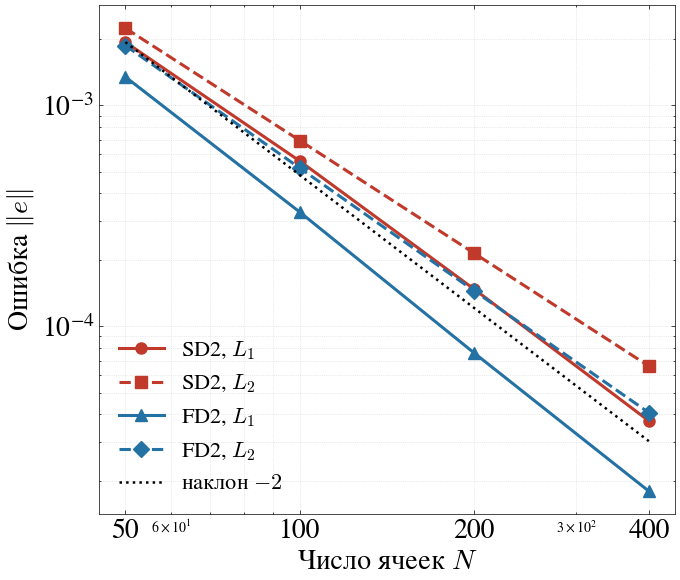
\includegraphics[width=\textwidth]{convergence_1d.png}
				\caption{\smaller{Ошибка по плотности $\rho$. Гладкая
						задача, $t=1$.}}
			\end{figure}
		\end{column}
		
		%--- ПРАВО: задача + таблица + вывод ---
		\begin{column}{0.48\textwidth}
			\footnotesize
			\textbf{Тест:} перенос гладкого профиля плотности
			\[
			\rho(x,0)=1+0.2\sin(2\pi x),\quad u=1,\ p=1,
			\]
			\[
			\rho(x,t)=1+0.2\sin\!\big(2\pi(x-t)\big).
			\]
			\vspace{-0.5cm}
			\begin{table}[h]
				\centering
				\caption{\smaller{Эмпирический порядок сходимости $r$ ($N{:}\,200{\to}400$)}}
				\vspace{-0.2cm}
				\resizebox{0.7\textwidth}{!}{%
					\begin{tabular}{lcc}
						\toprule
						Схема & $r_{L_1}$ & $r_{L_2}$ \\
						\midrule
						SD2 & 1.98 & 1.70 \\
						FD2 & 2.08 & 1.83 \\
						\bottomrule
					\end{tabular}
				}
			\end{table}
			%				\vspace{-0.3cm}
			%				\begin{alertblock}{}
				%					\smaller Обе схемы сходятся \textbf{близко ко 2-му порядку}.
				%					Снижение $p_{L_2}$ у SD2 --- особенность центральных схем
				%					(диссипация потока Лакса--Фридрихса), а не ошибка реализации.
				%					Формальный 2-й порядок подтверждён на 2D-вихре ($p\approx2$).
				%				\end{alertblock}
		\end{column}
	\end{columns}
	
\end{frame}
	

	%==================================================================
	% Слайд: 1D результаты + кросс-верификация
	\begin{frame}{Численное решение: одномерная постановка}

		\begin{figure}[!h]
			\begin{minipage}[t]{0.27\textwidth}
				\centering
				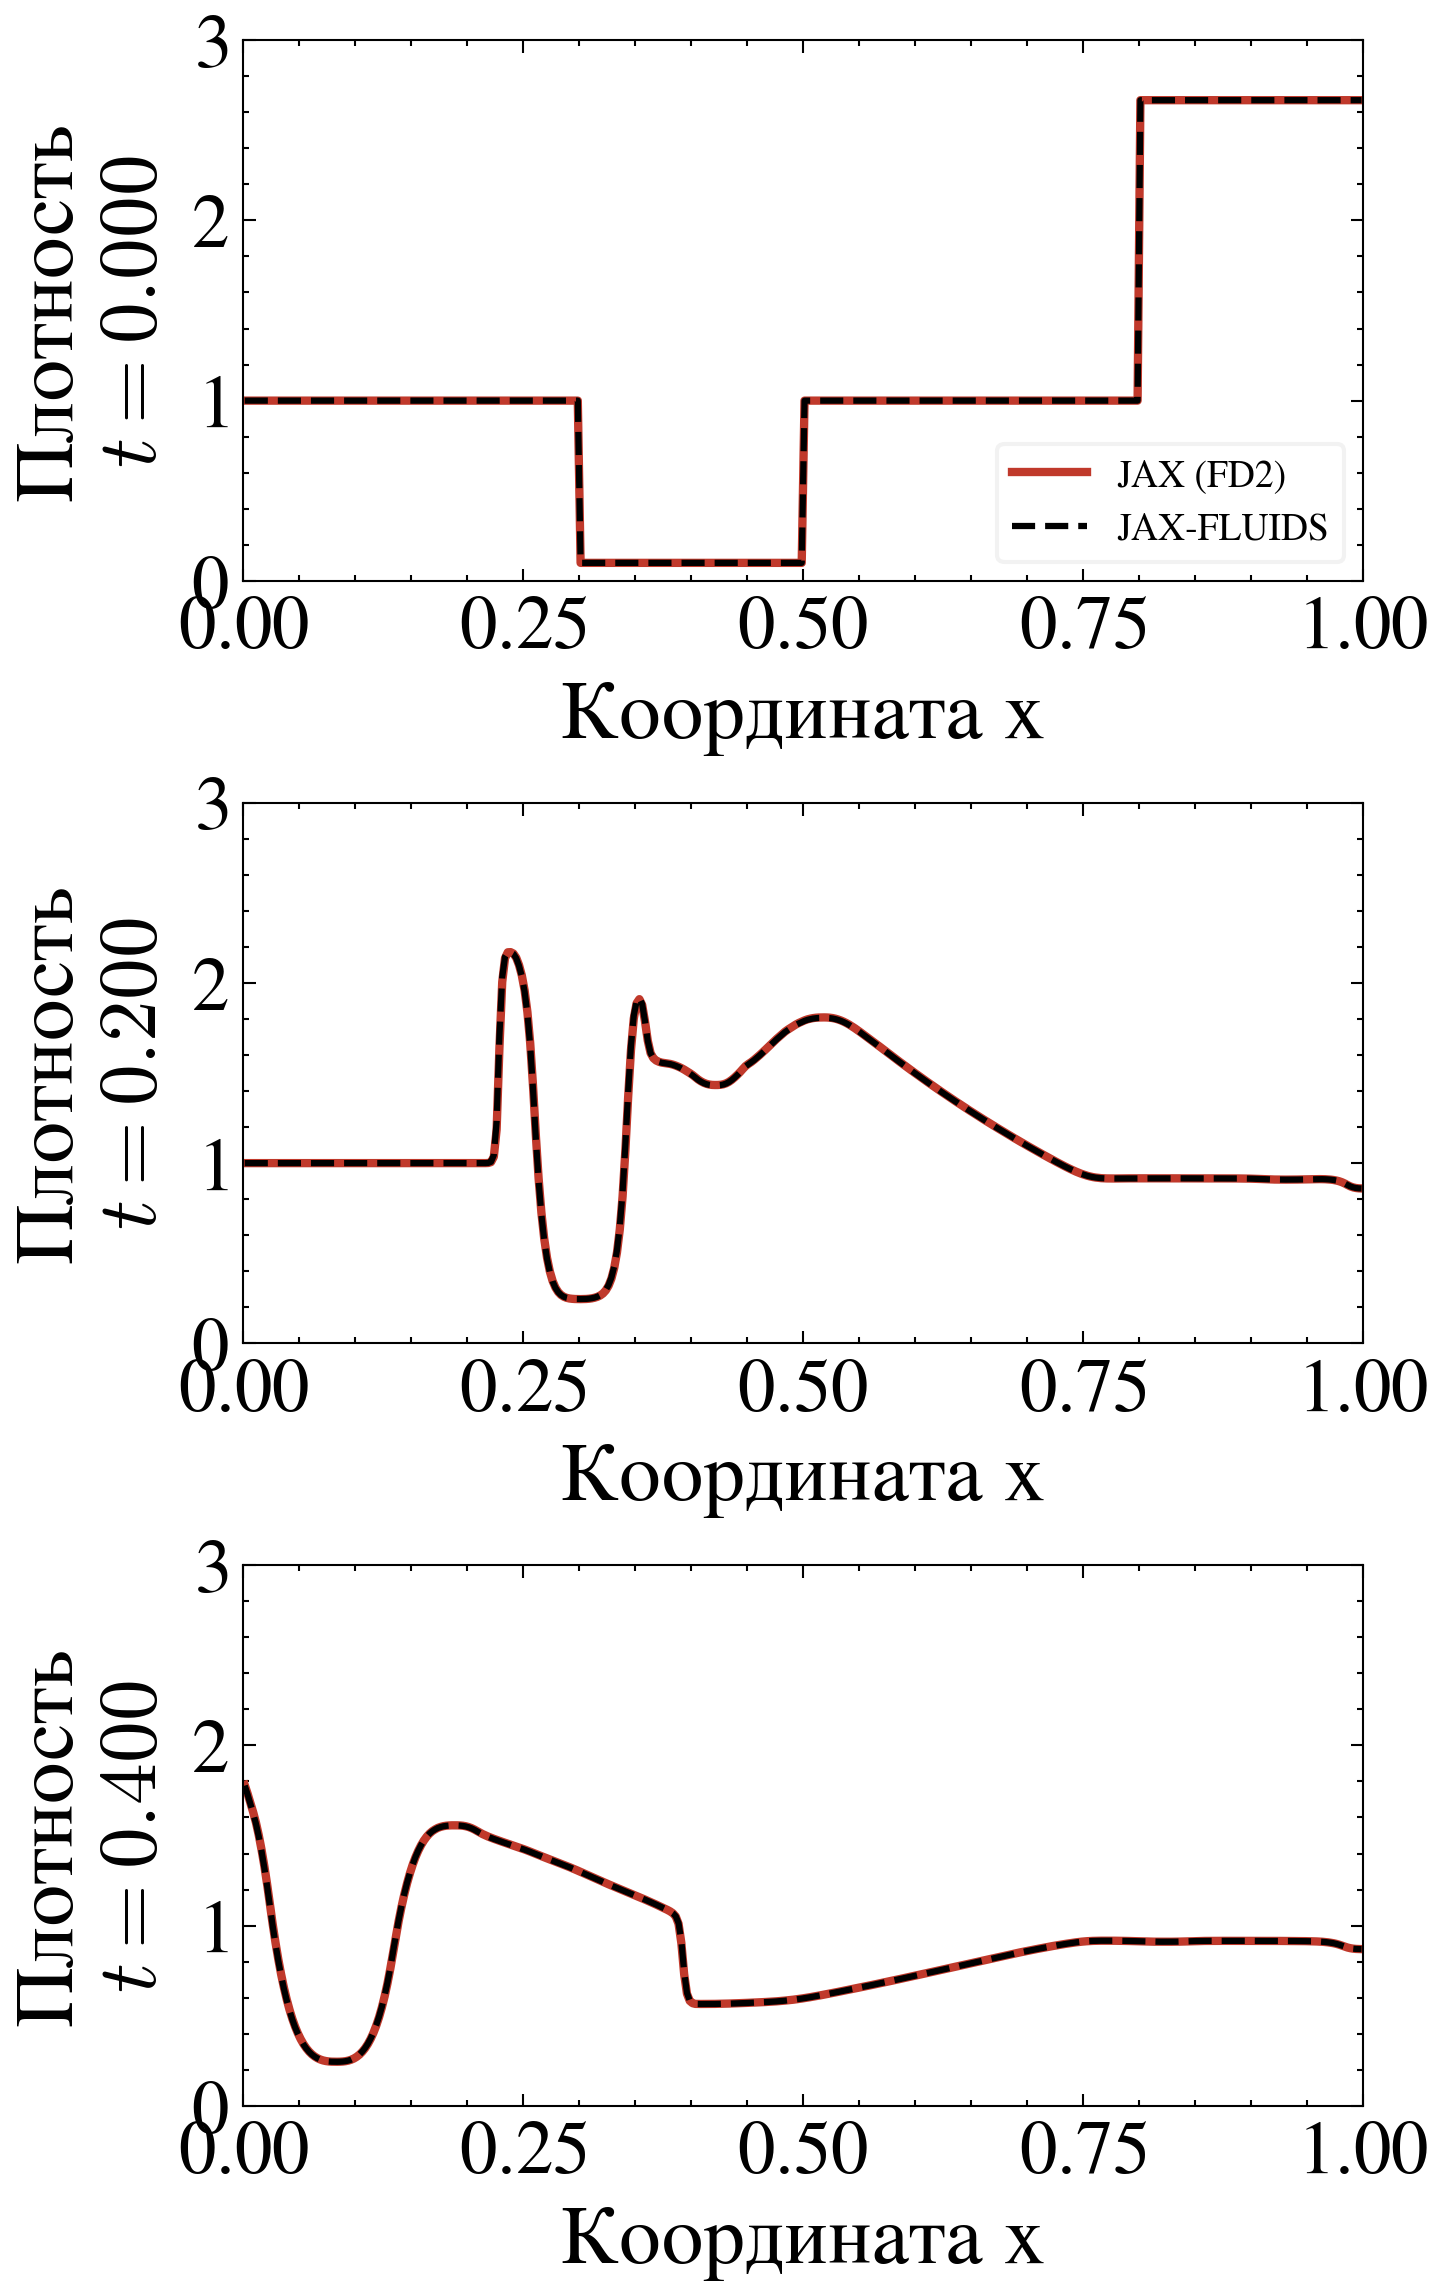
\includegraphics[width=1.06\textwidth]{rho_for_presentation_sd2_1d.png}
				
				\vspace{-0.25 cm}
				
				\caption*{\smaller{а)}}
			\end{minipage}\hfill
			\begin{minipage}[t]{0.30\textwidth}
				\centering
				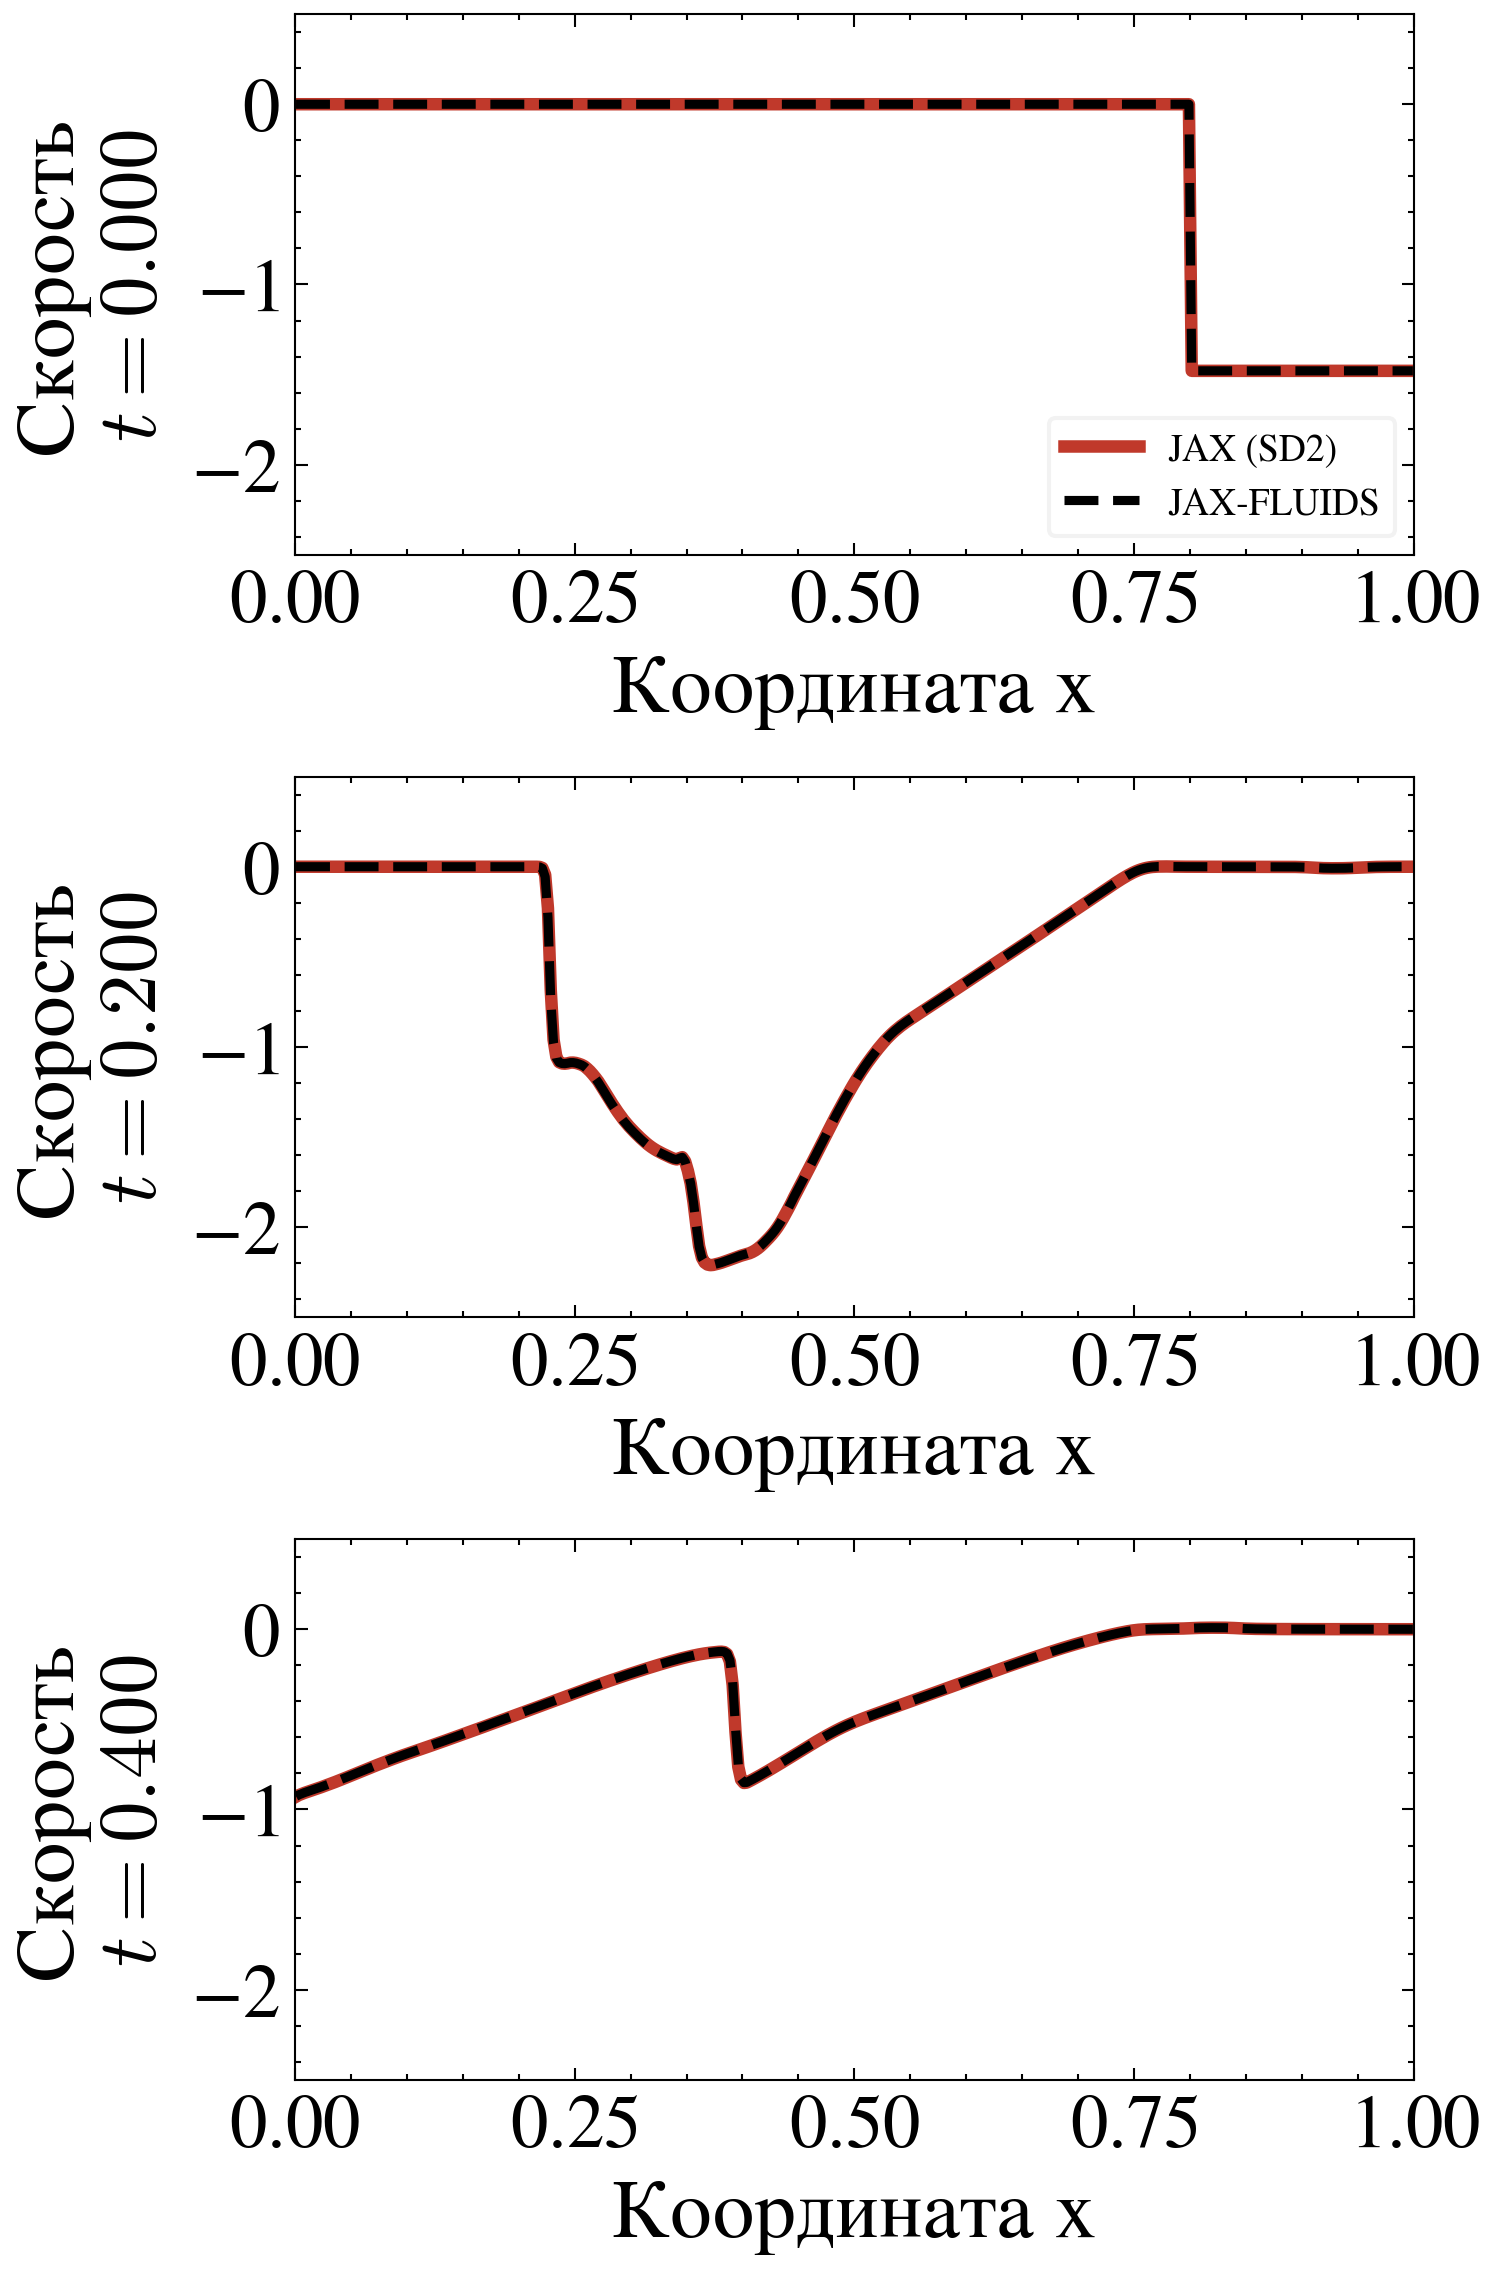
\includegraphics[width=\textwidth]{v_for_presentation_sd2_1d.png}
				
				\vspace{-0.25 cm}
				
				\caption*{\smaller{б)}}
			\end{minipage}\hfill
			\begin{minipage}[t]{0.29\textwidth}
				\centering
				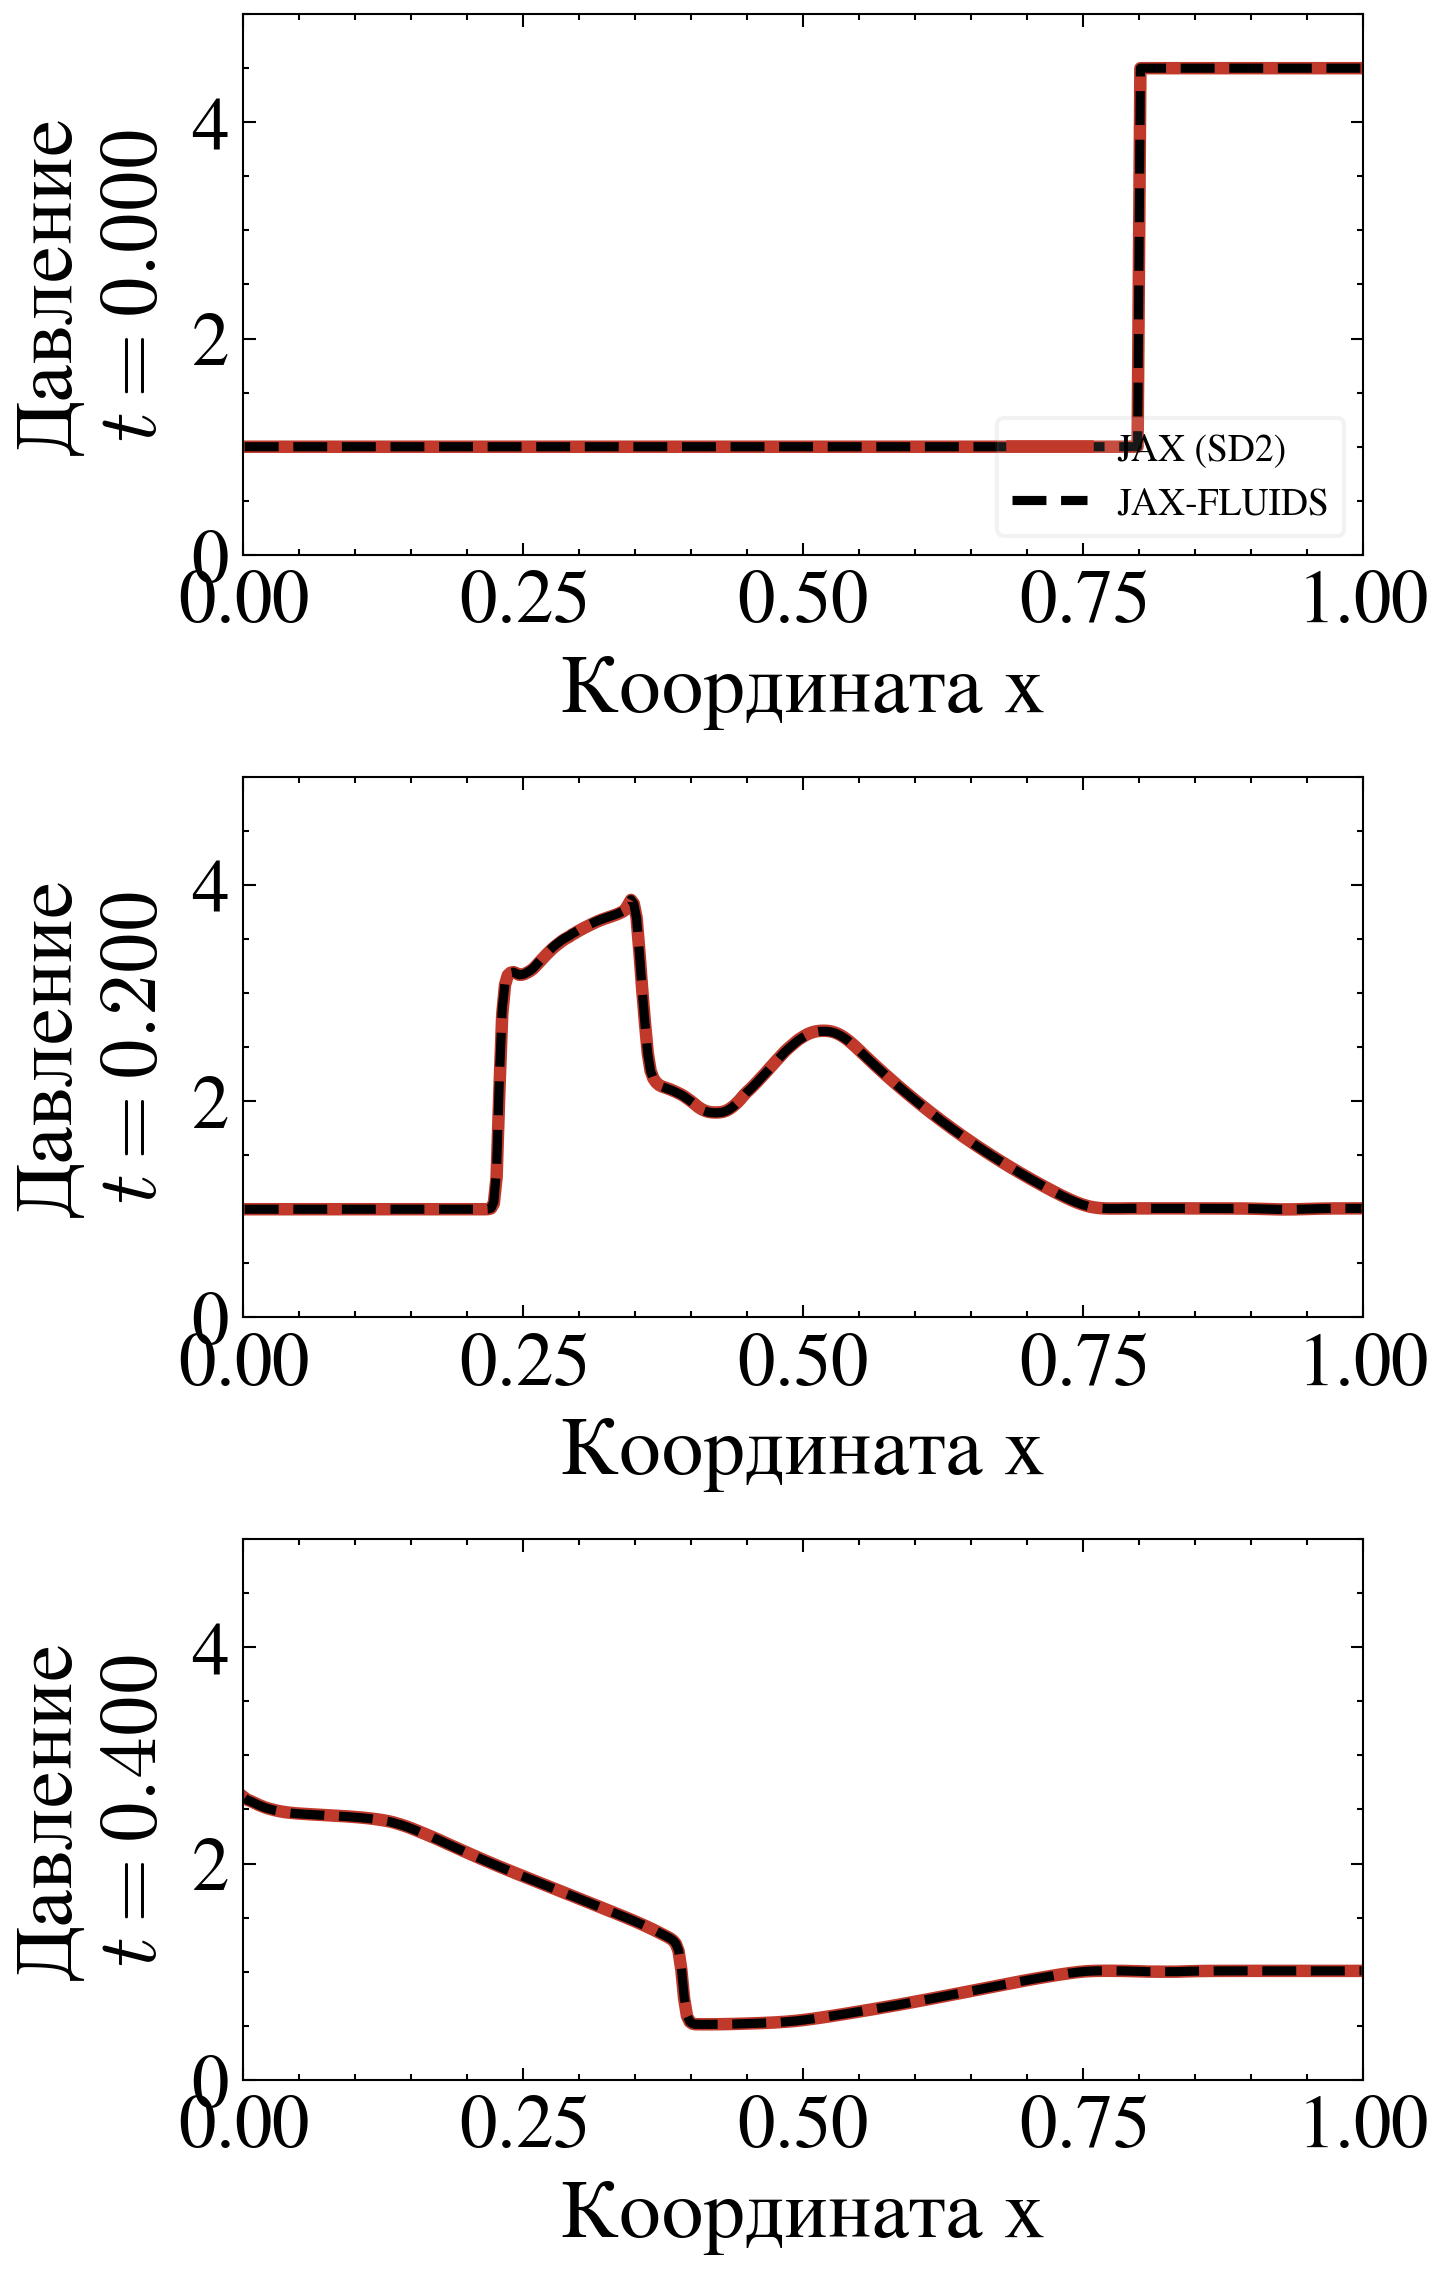
\includegraphics[width=\textwidth]{p_for_presentation_sd2_1d.png}
				
				\vspace{-0.25 cm}
				
				\caption*{\smaller{в)}}
			\end{minipage}
			\vspace{-0.5 cm}
			\caption{ \smaller{Эволюция примитивных переменных в модифицированной 1D задач Римана: а) плотность; б) скорость; в) давление (эталон JAX-FLUIDS)}}
		\end{figure}

	\end{frame}
	
	
	%==================================================================

%	%==================================================================
%	% Слайд: Производительность (числа из диплома, 2D)
%	\begin{frame}{Сравнительный анализ аппаратного ускорения: одномерная постановка}
%
%		\begin{columns}[c]
%			\begin{column}{0.5\textwidth}
%				\begin{figure}[h]
%					\centering
%					\vspace{-0.3 cm}
%					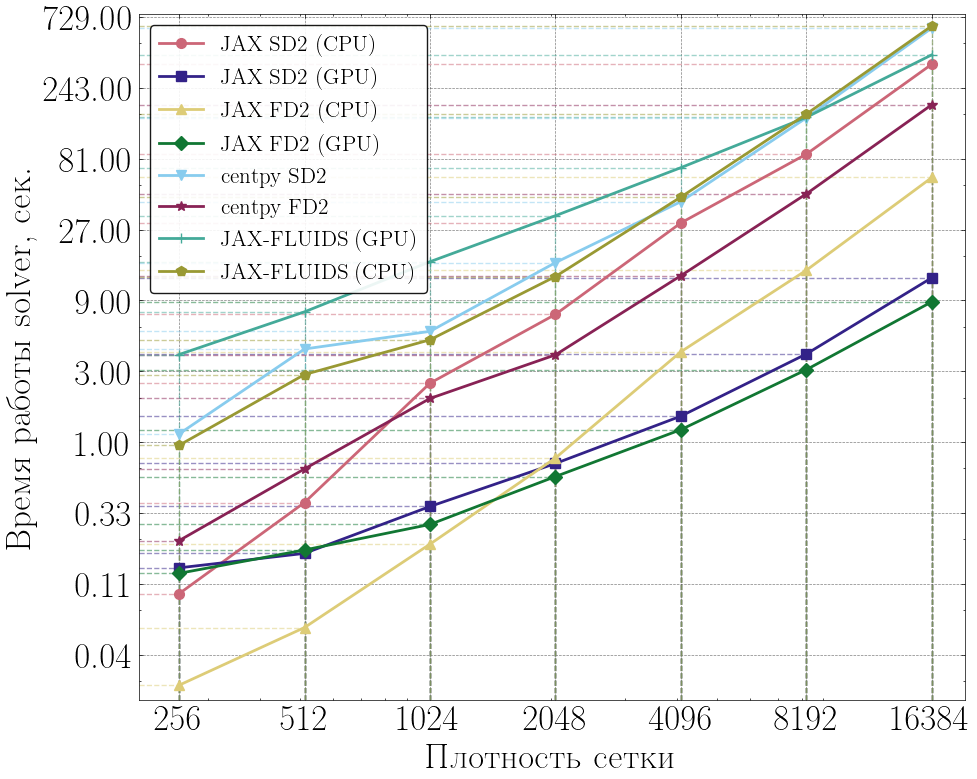
\includegraphics[width=\textwidth]{compare_time_plot_1d.png}
%					\caption{\smaller{Время счёта (с) от размера сетки $J$, 1D}}
%				\end{figure}
%			\end{column}
%			\begin{column}{0.5\textwidth}
%				\begin{table}[h]
%					\centering
%					\caption{\smaller{Время счёта (с), 1D}}
%					\vspace{-0.3 cm}
%					\resizebox{\textwidth}{!}{%
%						\begin{tabular}{lccccc}
%							\hline
%							$J$ & \texttt{centpy} & Разраб. CPU & Разраб. GPU & JAX-FL. CPU & JAX-FL. GPU \\
%							\hline
%							$\mathbf{256}$   & 1.138   & 0.096   & \textbf{0.143}  & 0.954   & 3.894 \\
%							$\mathbf{512}$   & 4.244   & 0.394   & \textbf{0.179}  & 2.857   & 7.545 \\
%							$\mathbf{1024}$  & 5.577   & 2.499   & \textbf{0.370}  & 4.893   & 16.403 \\
%							$\mathbf{2048}$  & 16.175  & 7.255   & \textbf{0.720}  & 13.040  & 33.451 \\
%							$\mathbf{4096}$  & 41.613  & 29.928  & \textbf{1.500}  & 44.688  & 70.443 \\
%							$\mathbf{8192}$  & 152.440 & 86.862  & \textbf{3.931}  & 161.556 & 153.630 \\
%							$\mathbf{16384}$ & 612.826 & 349.892 & \textbf{12.805} & 633.204 & 404.548 \\
%							\hline
%						\end{tabular}
%					}
%				\end{table}
%%				\vspace{-0.2cm}
%%				\begin{alertblock}{}
%%					\small GPU (1D, $J=16384$): до $\mathbf{47.9\times}$ быстрее \texttt{centpy} и $\mathbf{27.3\times}$ быстрее собственной CPU-версии. На малых 1D-сетках выигрыш GPU невелик из-за накладных расходов (закон $T\propto J^2$); полное преимущество раскрывается в 2D.
%%				\end{alertblock}
%			\end{column}
%		\end{columns}
%	\end{frame}
	
	%==================================================================
	% Слайд: Производительность (1D, схемы SD2 и FD2)
	\begin{frame}{Анализ аппаратного ускорения: одномерная постановка}
		
		\begin{columns}[c]
			\begin{column}{0.42\textwidth}
				\begin{figure}[h]
					\centering
					\vspace{-0.3 cm}
					\hspace*{-0.5cm}% <-- сдвиг графика влево
					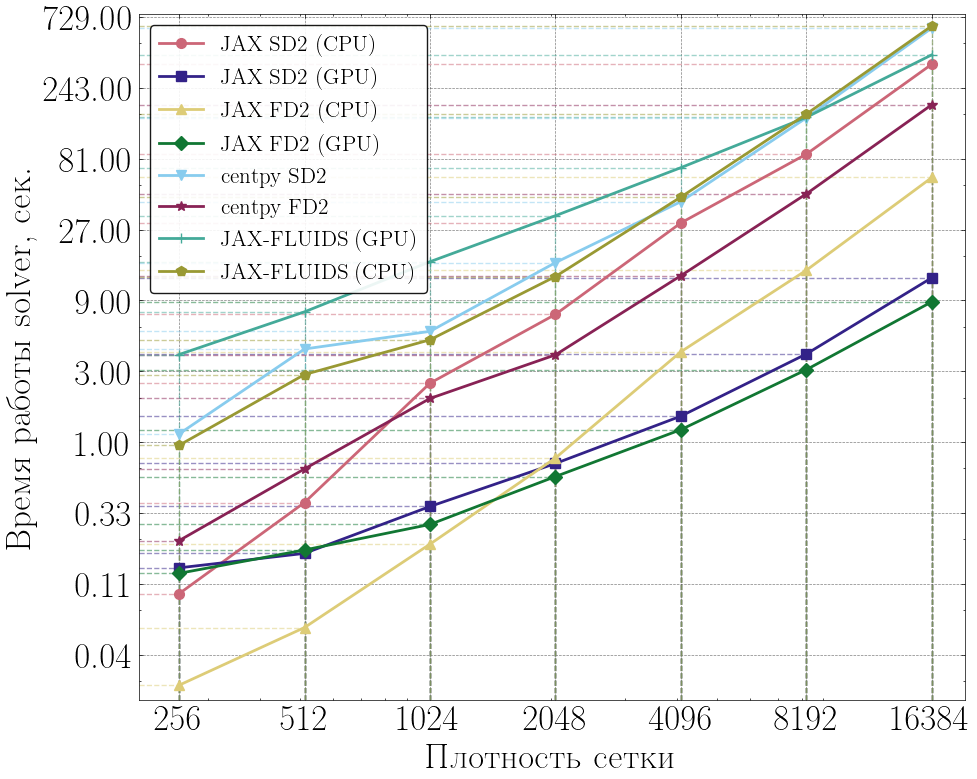
\includegraphics[width=1.12\textwidth]{compare_time_plot_1d.png}
					\caption{\smaller{Время счета (с), 1D}}
				\end{figure}
			\end{column}
			\begin{column}{0.58\textwidth}
				% ===== Основная таблица: SD2 + FD2 =====
				\begin{table}[h]
					\centering
					\caption{\smaller{Время счета (с), 1D, схемы SD2 и FD2}}
					\vspace{-0.3 cm}
					\resizebox{\textwidth}{!}{%
						\begin{tabular}{lcccccccc}
							\hline
							& \multicolumn{2}{c}{centpy}
							& \multicolumn{2}{c}{\tikzmark{tl}\textbf{JAX CPU}}
							& \multicolumn{2}{c}{\textbf{JAX GPU}}
							& \multicolumn{2}{c}{JAX-FL.} \\
							$J$ & SD2 & FD2 & \textbf{SD2} & \textbf{FD2} & \textbf{SD2} & \textbf{FD2} & CPU & GPU \\
							\hline
							$\mathbf{256}$   & 1.138   & 0.218   & \textbf{0.096}   & \textbf{0.023}  & \textbf{0.143}  & \textbf{0.131} & 0.954   & 3.894   \\
							$\mathbf{512}$   & 4.244   & 0.662   & \textbf{0.394}   & \textbf{0.057}  & \textbf{0.179}  & \textbf{0.189} & 2.857   & 7.545   \\
							$\mathbf{1024}$  & 5.577   & 1.972   & \textbf{2.499}   & \textbf{0.207}  & \textbf{0.370}  & \textbf{0.280} & 4.893   & 16.403  \\
							$\mathbf{2048}$  & 16.175  & 3.875   & \textbf{7.255}   & \textbf{0.785}  & \textbf{0.720}  & \textbf{0.588} & 13.040  & 33.451  \\
							$\mathbf{4096}$  & 41.613  & 13.218  & \textbf{29.928}  & \textbf{4.067}  & \textbf{1.500}  & \textbf{1.217} & 44.688  & 70.443  \\
							$\mathbf{8192}$\tikzmark{br}  & 152.440 & 46.947  & \textbf{86.862}  & \textbf{14.377} & \textbf{3.931}  & \textbf{3.082} & 161.556 & 153.630 \\
							$\mathbf{16384}$ & 612.826 & 186.817 & \textbf{349.892} & \textbf{60.462} & \textbf{12.805} & \textbf{8.819} & 633.204 & 404.548 \\
							\hline
						\end{tabular}
					}
					\begin{tikzpicture}[remember picture, overlay]
						\draw[teal, very thick, rounded corners=2pt]
						([xshift=18pt, yshift=-18pt]pic cs:tl) rectangle ([xshift=48pt, yshift=8pt]pic cs:br);
					\end{tikzpicture}
				\end{table}
				
				\vspace{-0.2cm}
				% ===== Вторая таблица: ускорение Разраб. GPU =====
				\begin{table}[h]
					\centering
					\caption{\smaller{Ускорение JAX GPU (1D, $J=16384$)}}
%					\vspace{-0.3 cm}
					\resizebox{0.85\textwidth}{!}{%
						\begin{tabular}{lcc}
							\hline
							Сравнение & SD2 & FD2 \\
							\hline
							JAX CPU        & 27.3$\times$          & 6.9$\times$  \\
							\tikzmark{tlc} centpy & \textbf{47.9$\times$} & \textbf{21.2$\times$} \tikzmark{brc} \\
							JAX-FLUIDS GPU & 31.6$\times$          & 45.9$\times$ \\
							\hline
						\end{tabular}
					}
					\begin{tikzpicture}[remember picture, overlay]
						\draw[teal, very thick, rounded corners=2pt]
						([xshift=-7pt, yshift=10pt]pic cs:tlc) rectangle ([xshift=20pt, yshift=-4pt]pic cs:brc);
					\end{tikzpicture}
				\end{table}
			\end{column}
		\end{columns}
		
	\end{frame}

	%==================================================================
	% Слайд: 2D результаты (НОВЫЙ "вау"-слайд)
	\begin{frame}{Двумерная постановка задачи}

		\begin{block}{Система уравнений Эйлера (2D)}
			\[
			\partial_t \begin{pmatrix} \rho \\ \rho u \\ \rho v \\ \rho E \end{pmatrix} +
			\partial_x \begin{pmatrix} \rho u \\ \rho u^2 + p \\ \rho u v \\ (\rho E + p)u \end{pmatrix} +
			\partial_y \begin{pmatrix} \rho v \\ \rho u v \\ \rho v^2 + p \\ (\rho E + p)v \end{pmatrix} = 0
			\]
			с тем же уравнением состояния идеального газа $p = (\gamma - 1)\big(\rho E - \tfrac{1}{2}\rho (u^2 + v^2)\big)$, $\gamma = 1.4$,
		\end{block}
		
		\vspace{-0.1 cm}

		в расчетной области $(x, y) \in [0, 1]^2$, с кусочно-постоянными НУ
		\vspace{-0.15 cm}
		\[
		(\rho, u, v, p)|_{t=0} =
		\begin{cases}
			(1, 0, 0, 1), & \text{невозмущенный газ,} \\
			(\alpha \cdot 1, 0, 0, 1), & \text{зоны энерговложения,} \\
			(2.667, -1.479, 0, 4.5), & \text{ударная волна: } x \in [0.8, 1].
		\end{cases}
		\]

		\vspace{-0.2 cm}
		Зоны энерговложения при $\alpha = 0.1$ --- круговая (центр $(0.45, 0.65)$, радиус $0.08$) и прямоугольная ($x \in [0.25, 0.41]$, $y \in [0.20, 0.44]$); слева  --- ГУ Неймана, остальные --- ГУ непротекания.

	\end{frame}
	
%	%==================================================================
%	% Слайд: Верификация (порядок точности)
%	\begin{frame}{Анализ сходимости: гладкое решение (поправить для 2D)}
%		\begin{block}{}
%			Для верификации теоретического второго порядка точности схемы SD2 проведено моделирование эволюции уравнения линейного переноса.
%			Порядок $p$ вычислялся методом экстраполяции Ричардсона с шагом измельчения $r=2$.
%		\end{block}
%		
%		\begin{table}[h]
%			\centering
%			\footnotesize
%			\renewcommand{\arraystretch}{1.3}
%			\begin{tabular}{lccc}
%				\hline
%				\textbf{Переменная} & \textbf{Ошибка (100$\to$200)} & \textbf{Ошибка (200$\to$400)} & \textbf{Порядок $p$} \\
%				\hline
%				$u(x, t)$ & $8.92 \times 10^{-4}$ & $2.09 \times 10^{-4}$ & \textbf{2.09} \\
%				\hline
%			\end{tabular}
%		\end{table}
%		
%		\begin{columns}[c]
%			\begin{column}{0.55\textwidth}
%				\[
%				E = \|\mathbf{u}^{2h} - \mathbf{u}^{h}\|_{L_1} = \frac{1}{L} \sum_i |u_i^{2h} - u_i^h| \cdot \Delta x
%				\]
%				\[
%				p = \log_2 \left( \frac{|| \mathbf{u}^{4h} - \mathbf{u}^{2h} ||_{L_1}}{|| \mathbf{u}^{2h} - \mathbf{u}^{h} ||_{L_1}} \right)
%				\]
%			\end{column}
%			\begin{column}{0.45\textwidth}
%				\footnotesize
%				Неосцилляторность дополнительно подтверждена:
%				\begin{itemize}
%					\item контролем полной вариации $\mathrm{TV}(t)$ (1D);
%					\item выполнением принципа максимума (2D).
%				\end{itemize}
%			\end{column}
%		\end{columns}
%		
%	\end{frame}
	
	
%	%==================================================================
%	\begin{frame}{Сходимость в 2D: изоэнтропийный вихрь Ху--Шу}
%		
%		\begin{columns}[c]
%			%--- ЛЕВО: парный log-log график ---
%			%\hspace*{-1.5cm}% <-- сдвиг графика влево
%			\begin{column}{0.5\textwidth}
%				\begin{figure}[h]
%					\centering
%					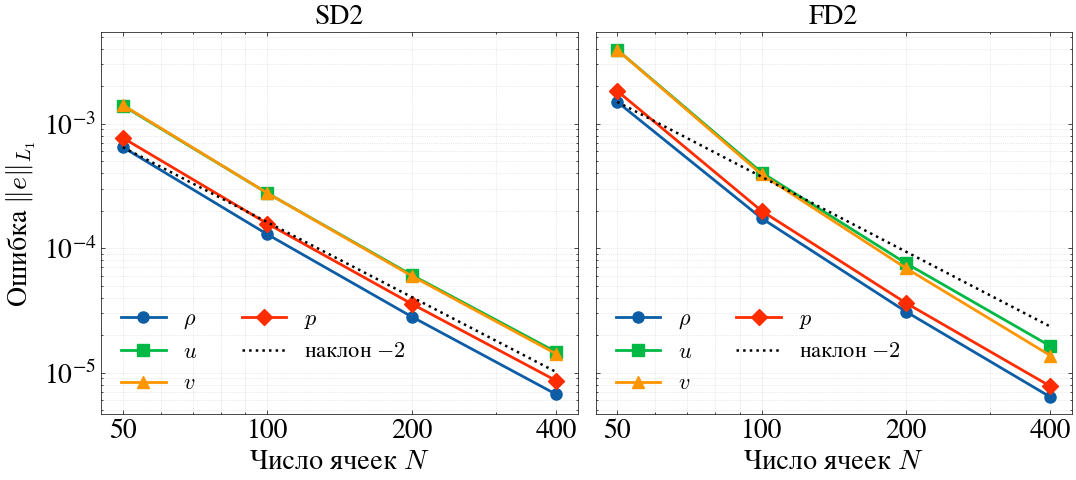
\includegraphics[width=0.7\textwidth]{convergence_2d_L1.png}
%					\caption{\smaller{Ошибка по $L_1$ для $\rho,u,v,p$, $t=1$.}}
%				\end{figure}
%			\end{column}
%			
%			%--- ПРАВО: задача + таблица + вывод ---
%			\begin{column}{0.5\textwidth}
%				\footnotesize
%				\textbf{Тест:} перенос гладкого изоэнтропийного вихря
%				($\varepsilon=5$) на $[0,10]^2$, периодич. ГУ.
%				\vspace{0.1cm}
%				\begin{table}[h]
%					\centering
%					\caption{\smaller{Порядок $p$ ($N{:}\,200{\to}400$)}}
%					\vspace{-0.2cm}
%					\resizebox{0.7\textwidth}{!}{%
%						\begin{tabular}{lcccc}
%							\toprule
%							\multirow{2}{*}{Перем.} & \multicolumn{2}{c}{SD2} & \multicolumn{2}{c}{FD2} \\
%							\cmidrule(lr){2-3}\cmidrule(lr){4-5}
%							& $p_{L_1}$ & $p_{L_2}$ & $p_{L_1}$ & $p_{L_2}$ \\
%							\midrule
%							$\rho$ & 2.07 & 2.06 & 2.28 & 2.29 \\
%							$u$    & 2.06 & 2.08 & 2.21 & 2.26 \\
%							$v$    & 2.08 & 2.09 & 2.33 & 2.38 \\
%							$p$    & 2.05 & 2.07 & 2.22 & 2.30 \\
%							\bottomrule
%						\end{tabular}
%					}
%				\end{table}
%%				\begin{alertblock}{}
%%					\smaller \textbf{2-й порядок по всем переменным} и по обеим
%%					нормам. В отличие от 1D, $L_2$ \emph{не проседает} — гладкий
%%					вихрь и неогранич. реконструкция. Расщепление по направлениям
%%					(\texttt{jax.numpy}) сохраняет точность схемы.
%%				\end{alertblock}
%			\end{column}
%		\end{columns}
%		
%	\end{frame}
	
	
	
%		%==================================================================
%	% Слайд: 1D результаты + кросс-верификация
%	\begin{frame}{Численное решение: двумерная постановка}
%		
%		\begin{figure}[!h]
%			\begin{minipage}[t]{0.27\textwidth}
%				\centering
%				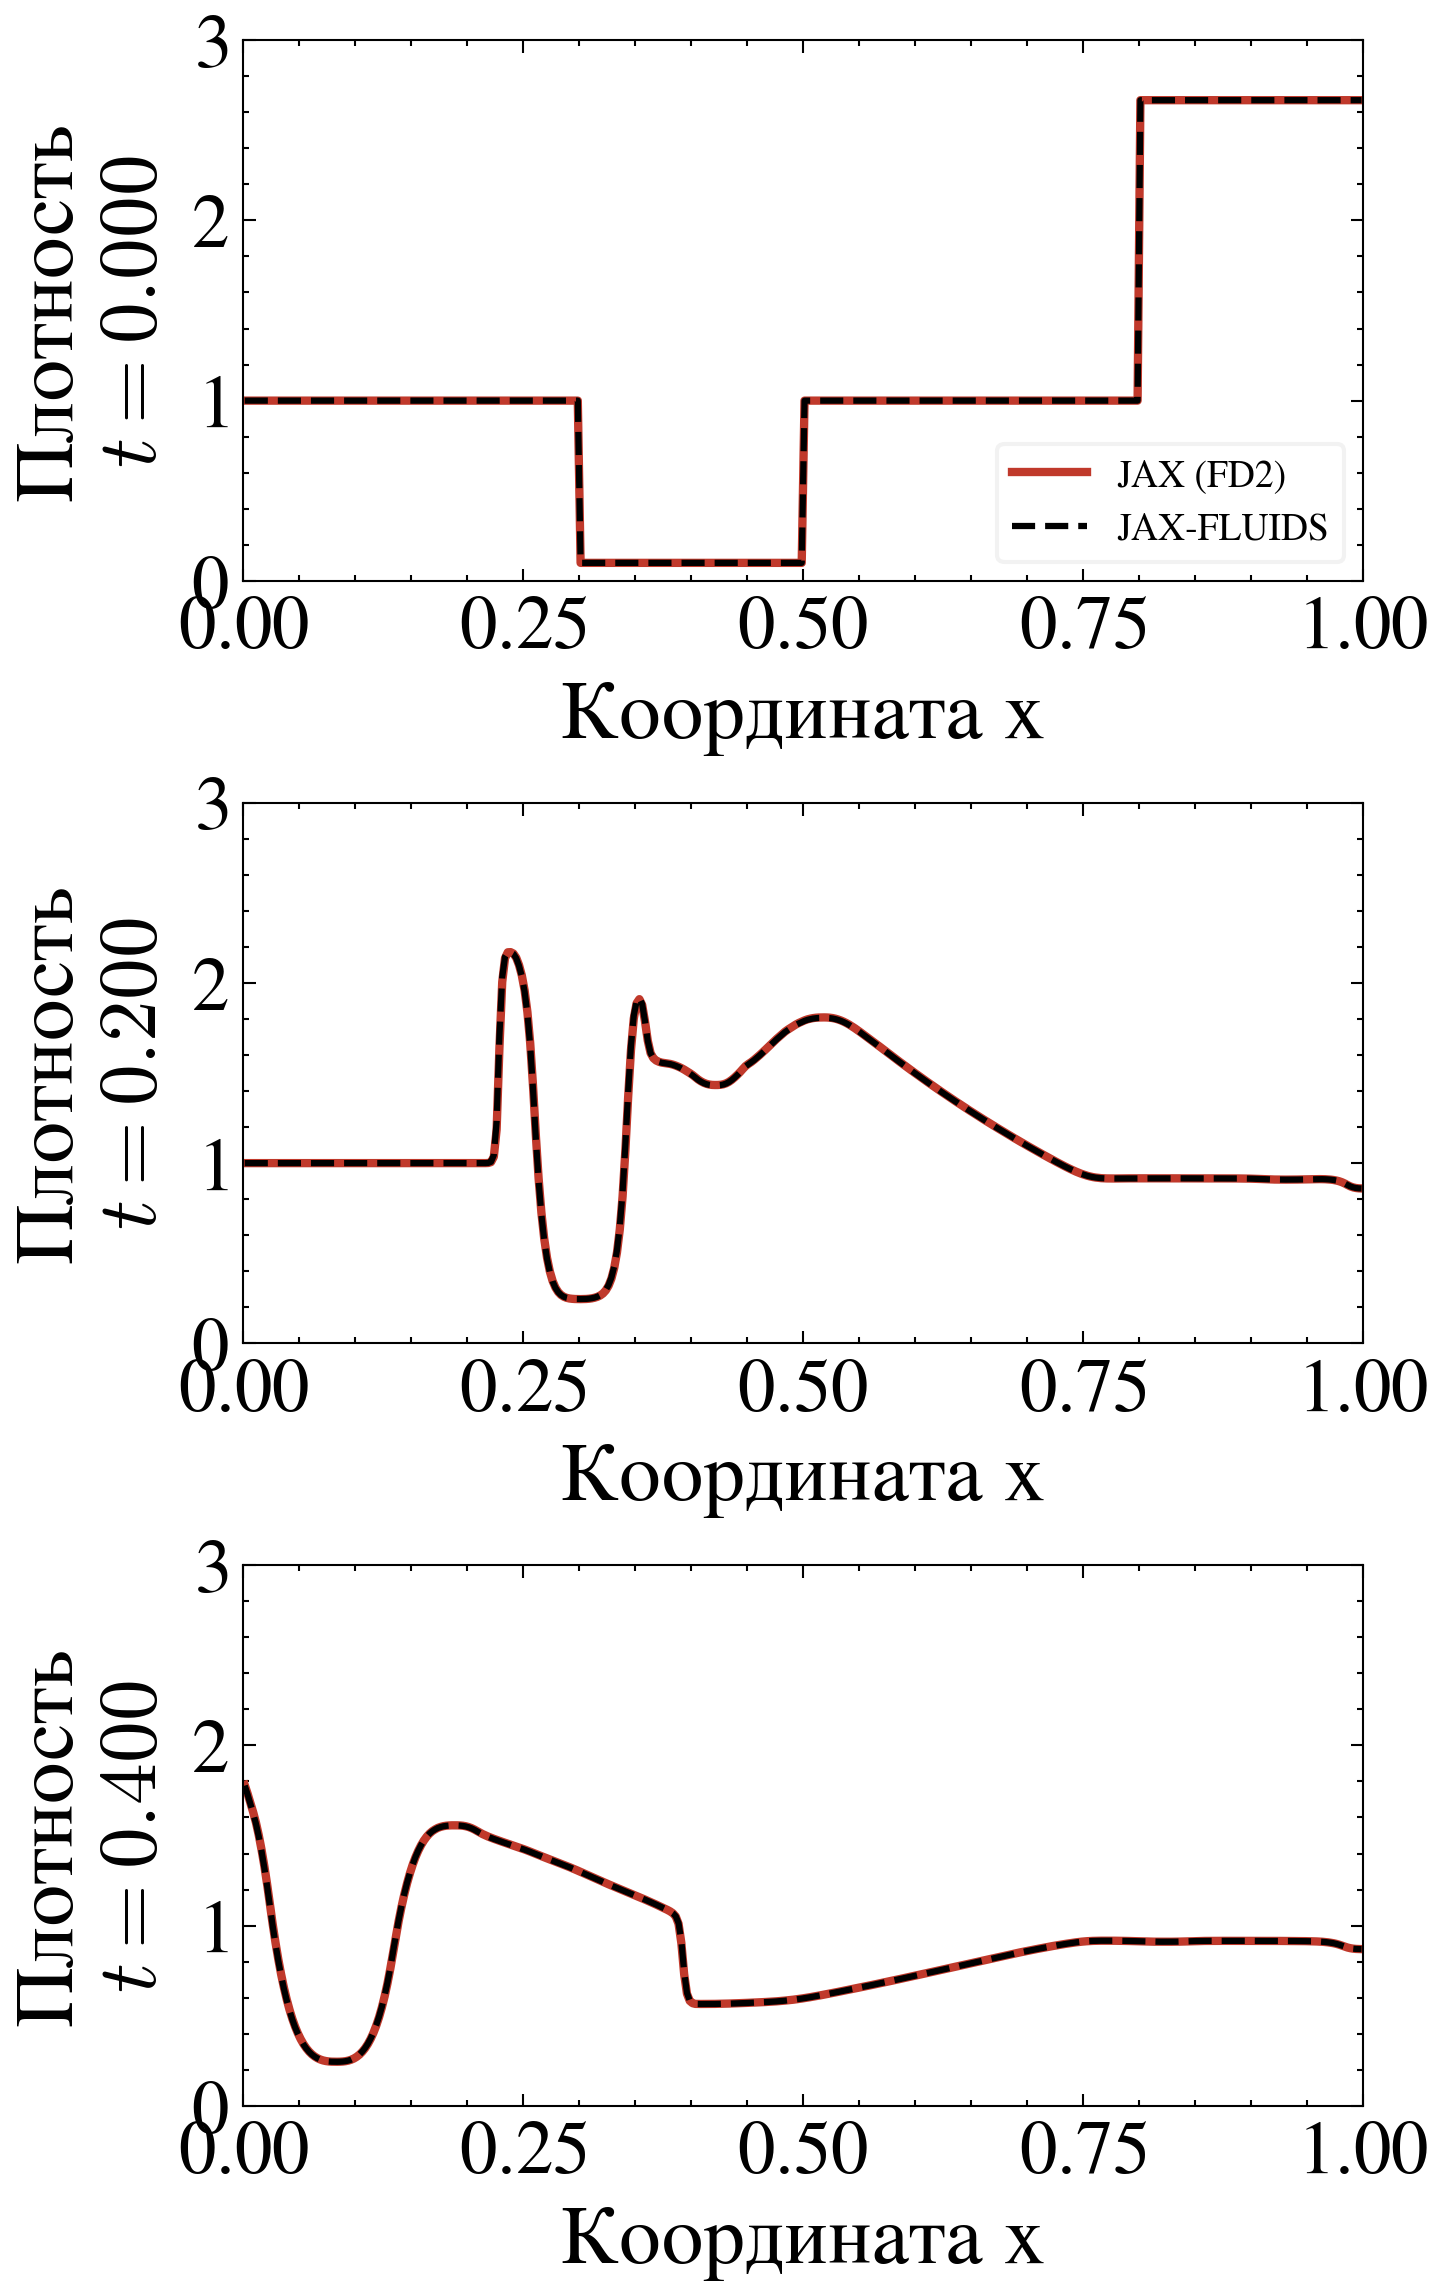
\includegraphics[width=1.06\textwidth]{rho_for_presentation_sd2_1d.png}
%				
%				\vspace{-0.25 cm}
%				
%				\caption*{\smaller{(a)}}
%			\end{minipage}\hfill
%			\begin{minipage}[t]{0.30\textwidth}
%				\centering
%				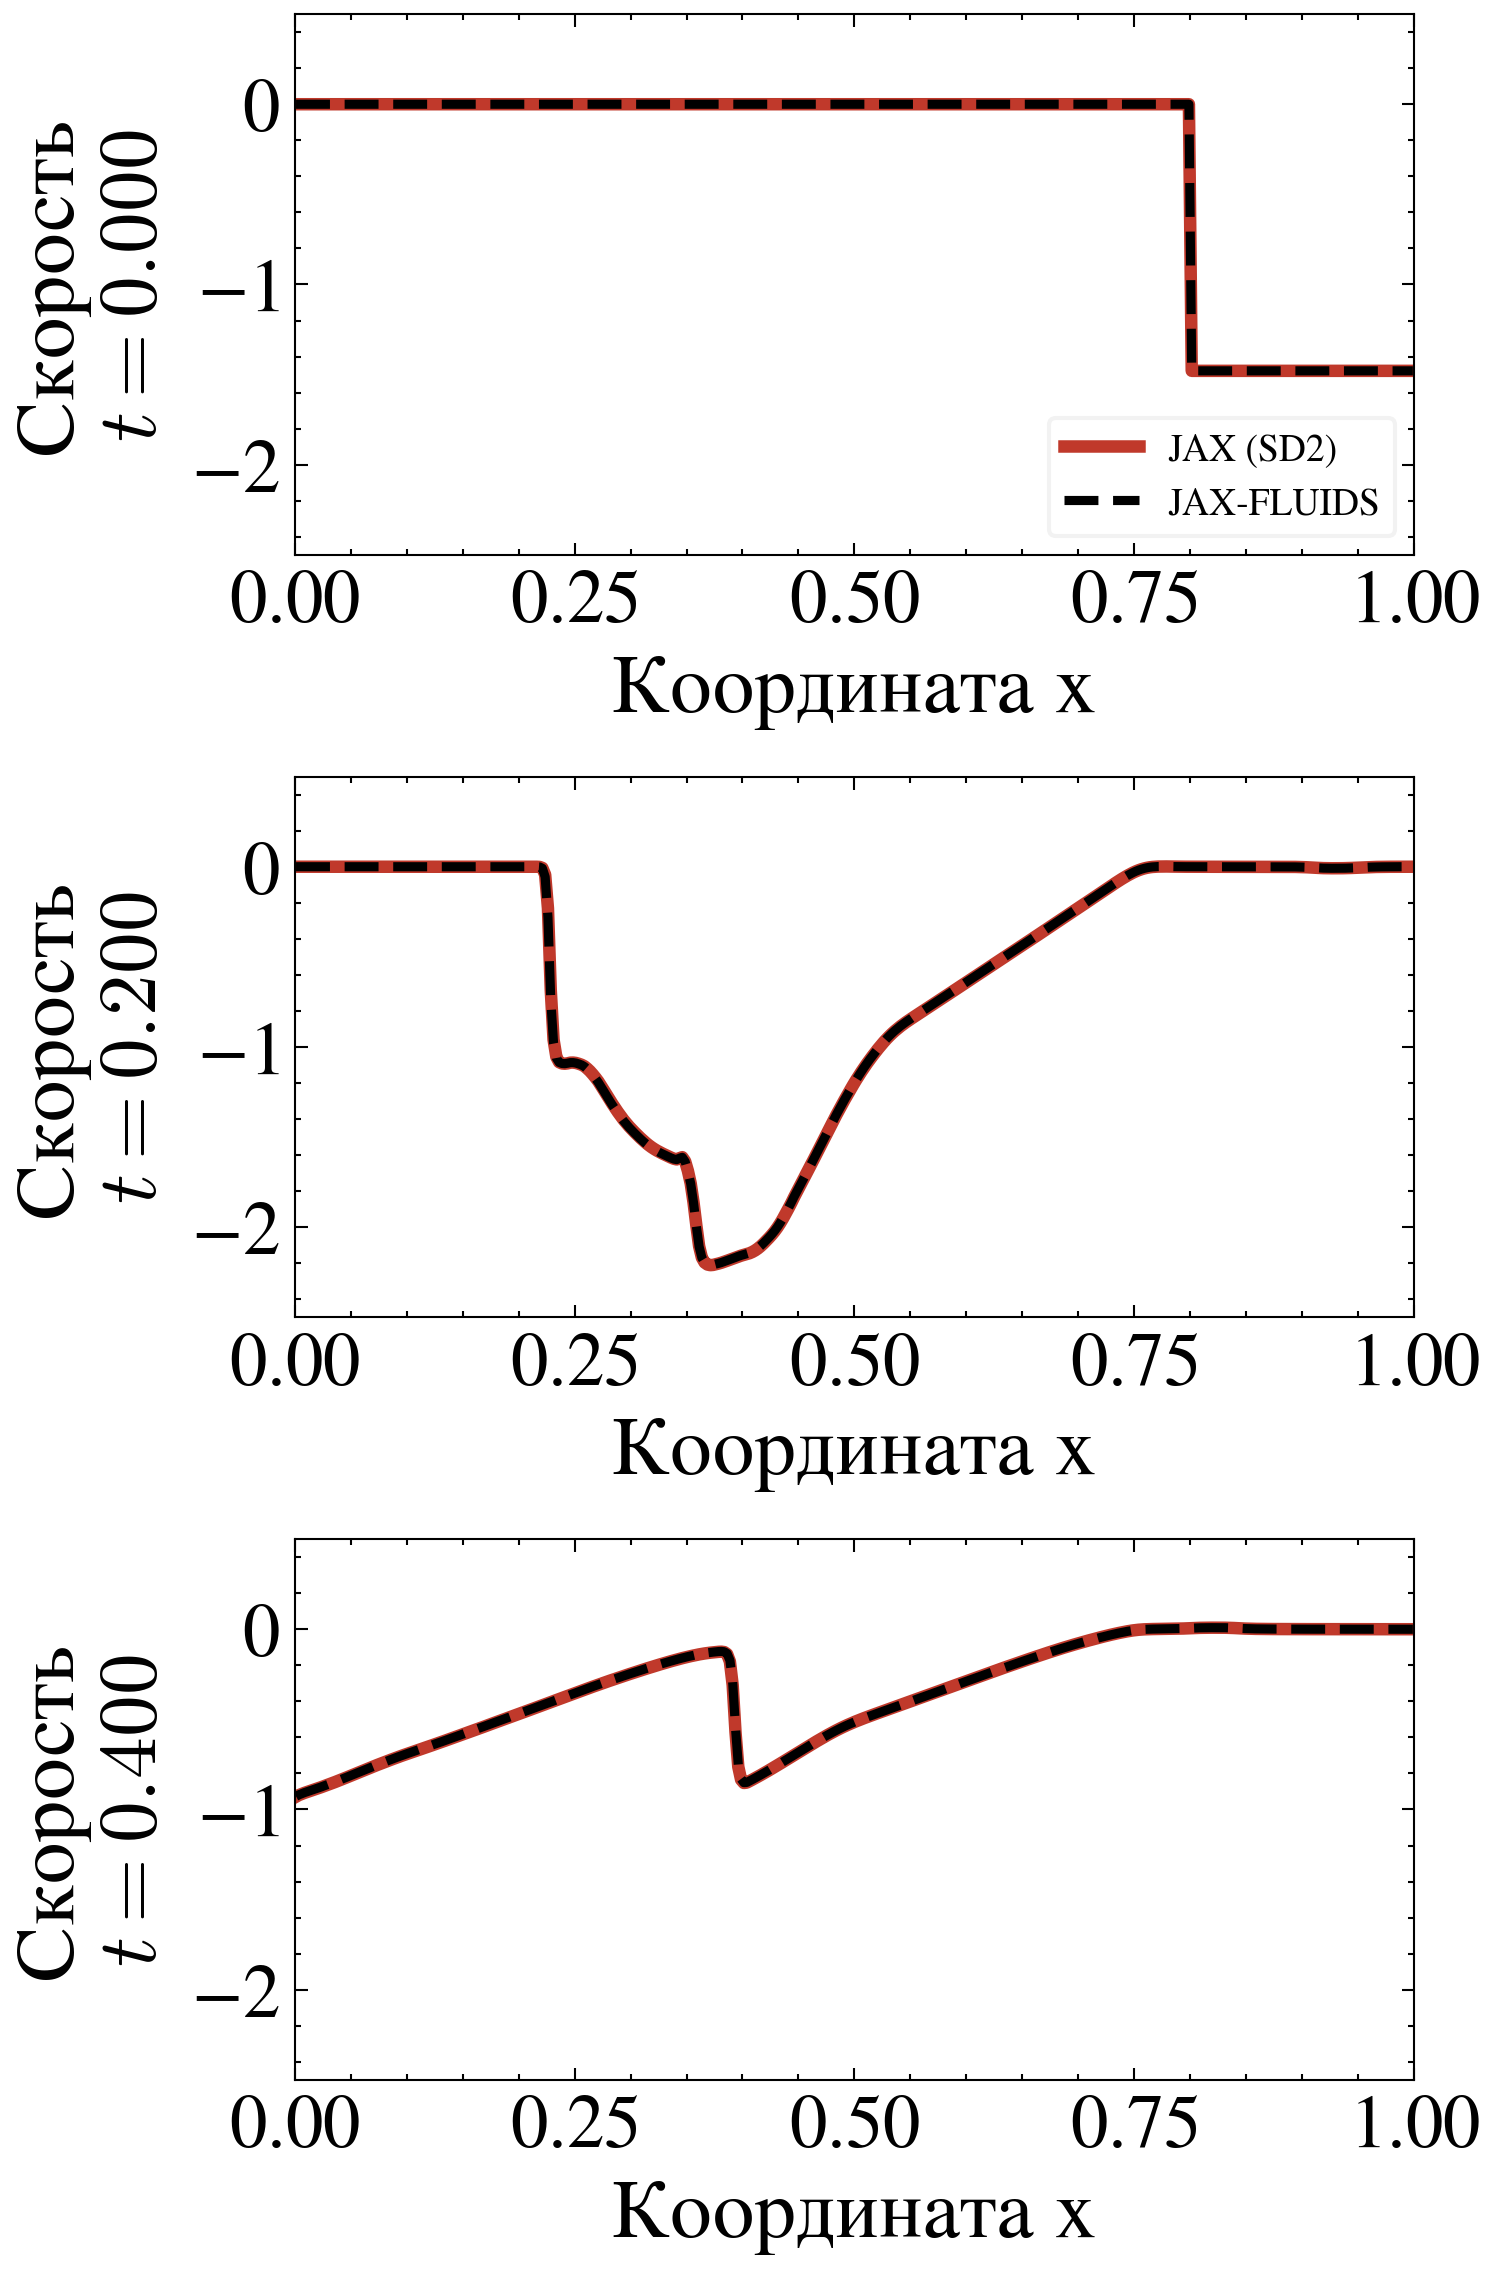
\includegraphics[width=\textwidth]{v_for_presentation_sd2_1d.png}
%				
%				\vspace{-0.25 cm}
%				
%				\caption*{\smaller{(b)}}
%			\end{minipage}\hfill
%			\begin{minipage}[t]{0.29\textwidth}
%				\centering
%				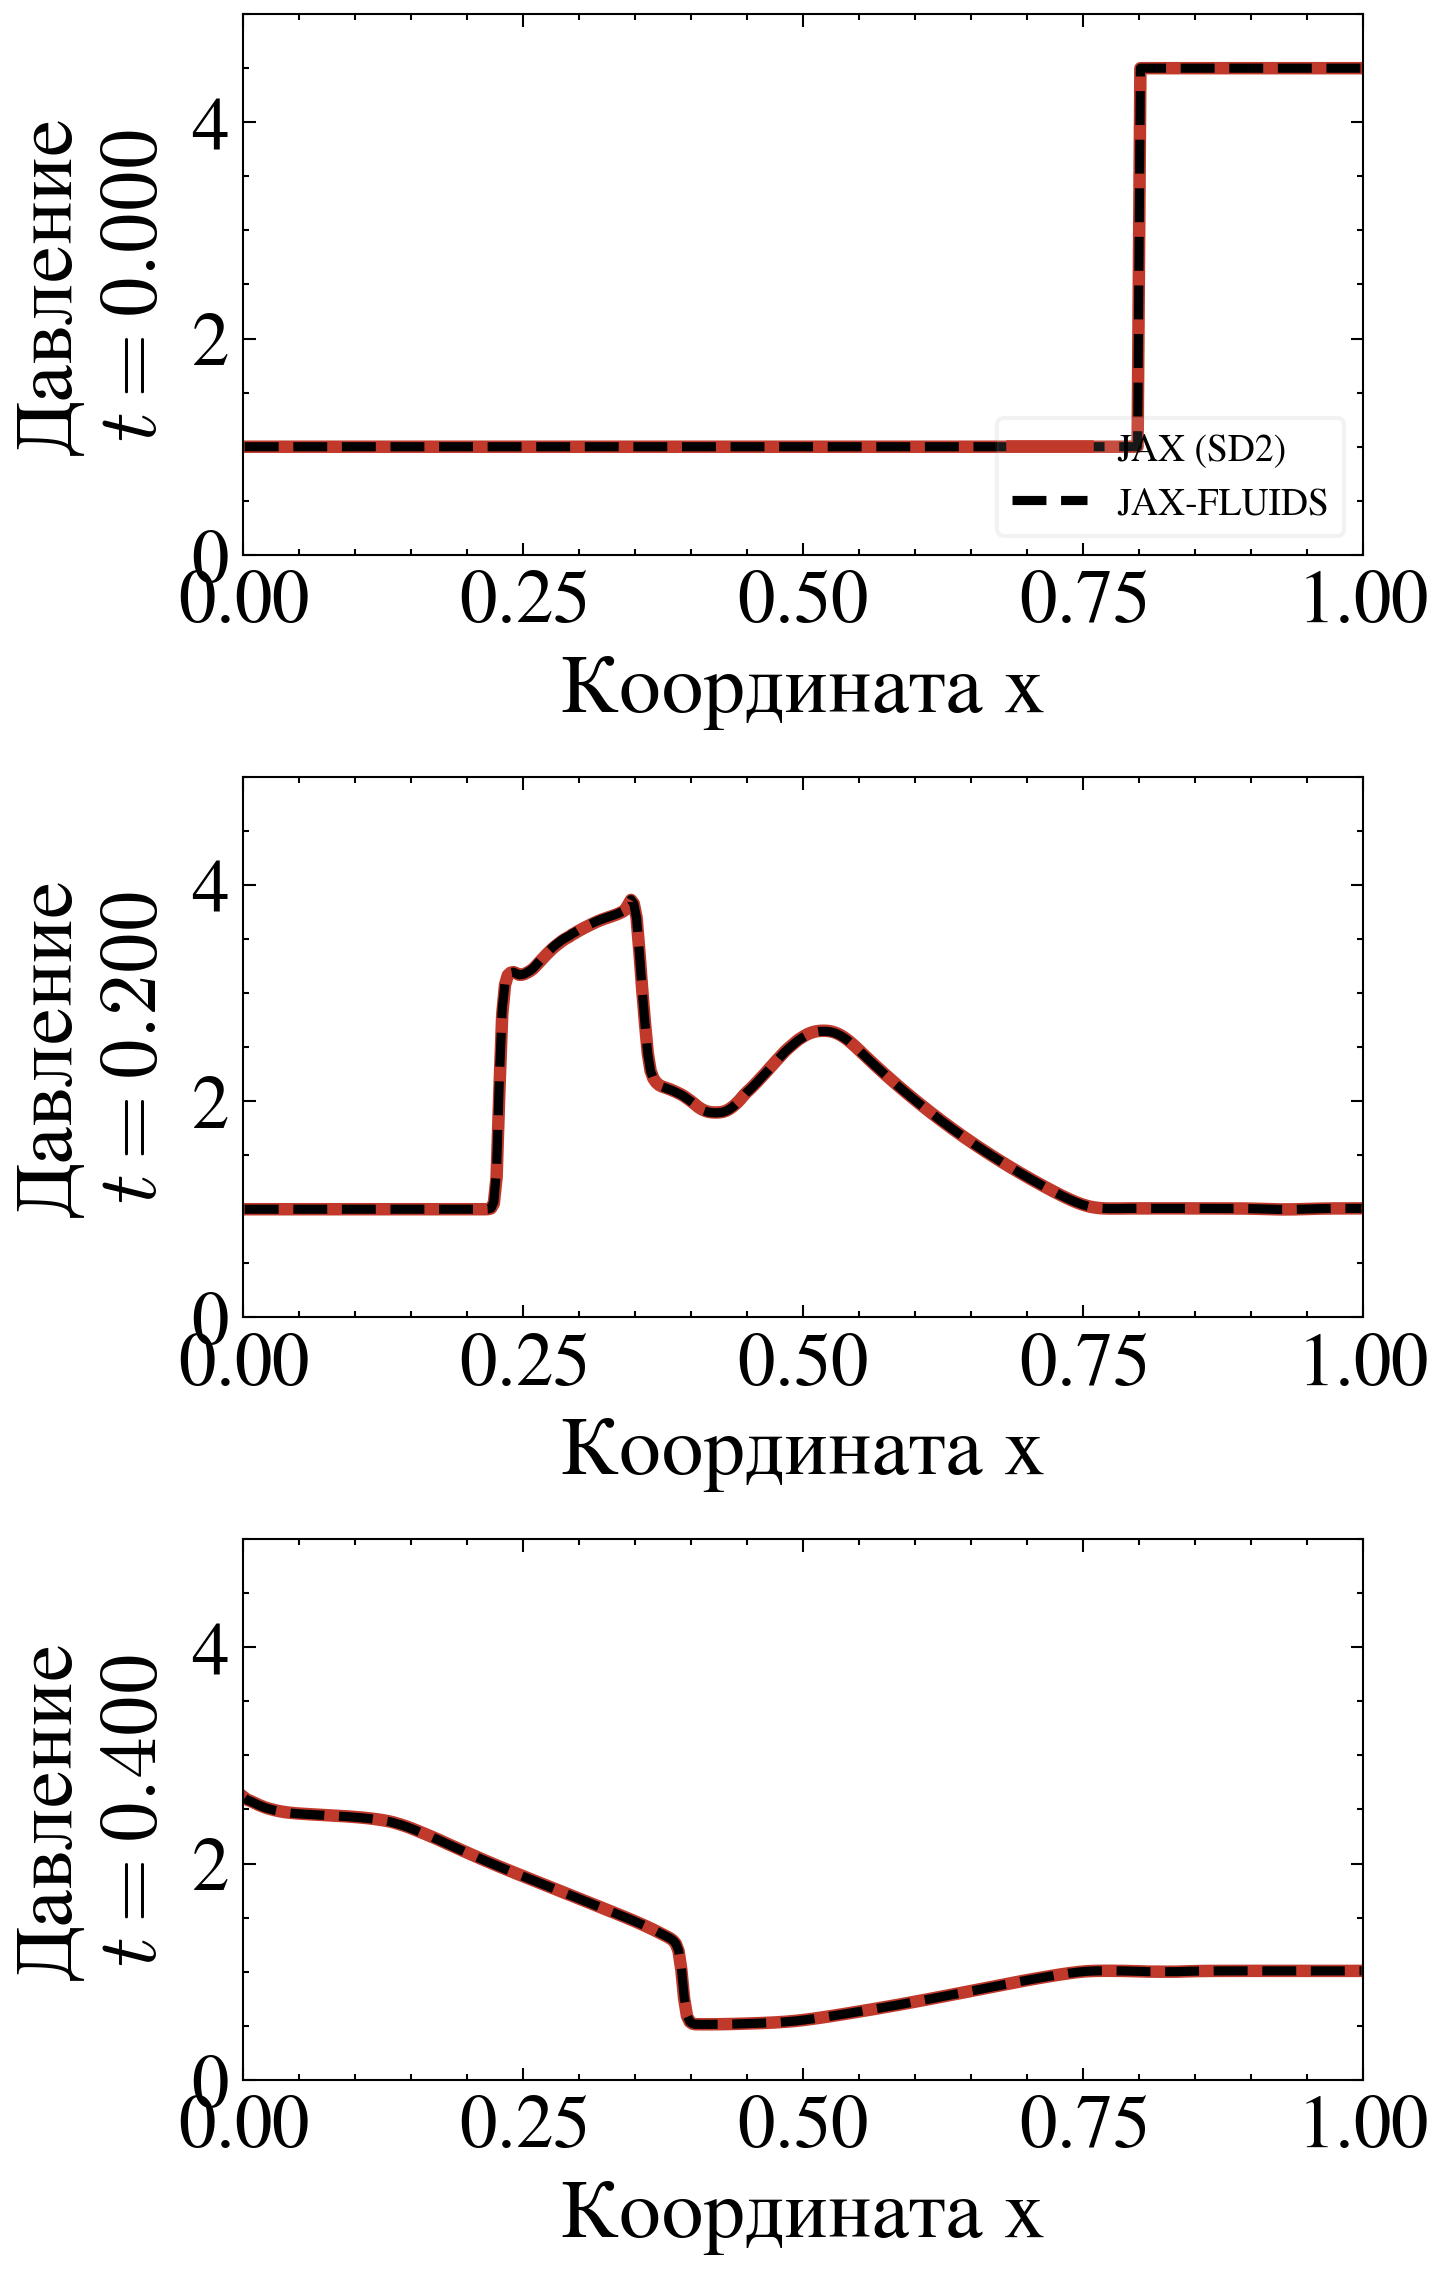
\includegraphics[width=\textwidth]{p_for_presentation_sd2_1d.png}
%				
%				\vspace{-0.25 cm}
%				
%				\caption*{\smaller{(c)}}
%			\end{minipage}
%			\vspace{-0.5 cm}
%			\caption{ \smaller{Эволюция примитивных переменных в модифицированной 1D задаче Римана: (a) Плотность; (b) Скорость; (c) Давление с наложением на эталон \texttt{JAX-FLUIDS}}}
%		\end{figure}
%		
%	\end{frame}
%	
%	%==================================================================
%	% Слайд: 2D плотность — начальное слева, сравнение методов справа
%	\begin{frame}{Двумерная постановка: эволюция плотности}
%		
%		% Удобная длина для размера одной ячейки сетки справа
%		\newlength{\cellw}\setlength{\cellw}{0.205\textwidth}
%		
%		\begin{columns}[c]
%			%--- ЛЕВО: начальное условие на всю высоту ---
%			\begin{column}{0.30\textwidth}
%				\centering
%				\textbf{Начальное условие}\par
%				\vspace{0.2cm}
%				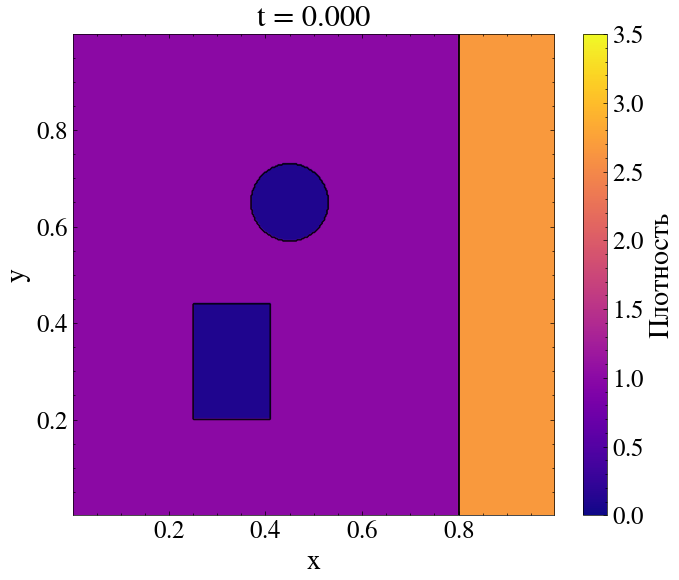
\includegraphics[width=\textwidth]{rieman_modify_2d_init_jax-fluids.png}\par
%				\vspace{0.2cm}
%				{\small $t = 0$}
%			\end{column}
%			
%			%--- ПРАВО: сетка 2x3 (время x метод) ---
%			\begin{column}{0.68\textwidth}
%				\centering
%				\setlength{\tabcolsep}{2pt}%
%				\renewcommand{\arraystretch}{0.6}%
%				\begin{tabular}{c ccc}
%					% --- заголовки столбцов: методы ---
%					& \textbf{SD2} & \textbf{FD2} & \textbf{JAX-FLUIDS} \\[2pt]
%					% --- строка 1: t = T/2 ---
%					\rotatebox{90}{\small $t = T/2$} &
%					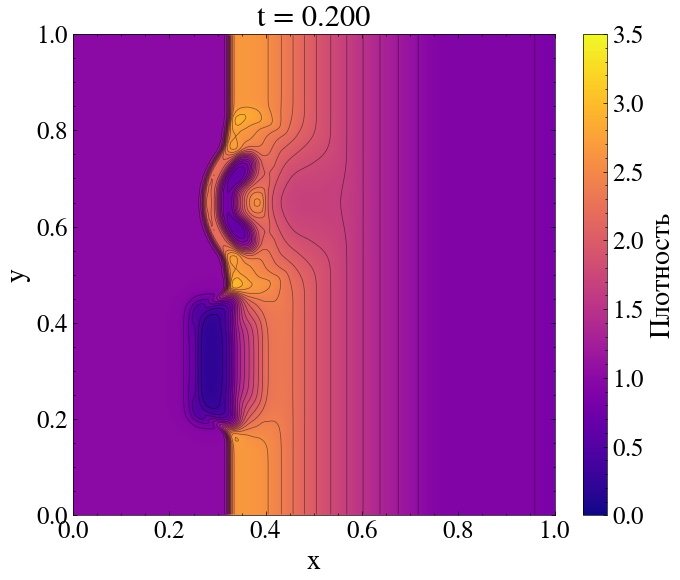
\includegraphics[width=\cellw]{rieman_modify_2d_half_jax_sd2.png} &
%					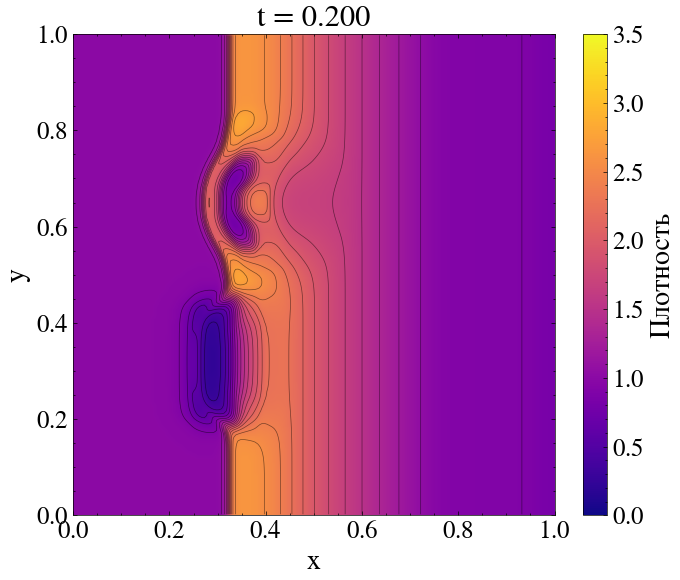
\includegraphics[width=\cellw]{rieman_modify_2d_half_jax_fd2.png} &
%					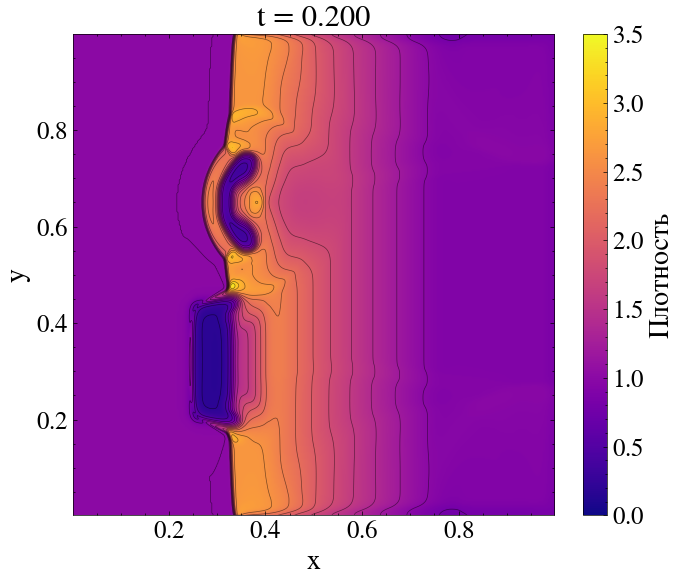
\includegraphics[width=\cellw]{rieman_modify_2d_half_jax-fluids.png} \\[2pt]
%					% --- строка 2: t = T ---
%					\rotatebox{90}{\small $t = T$} &
%					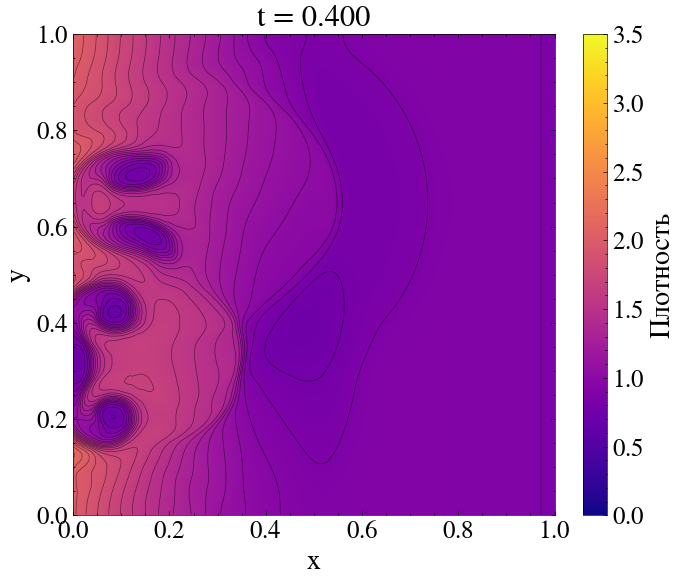
\includegraphics[width=\cellw]{rieman_modify_2d_final_jax_sd2.png} &
%					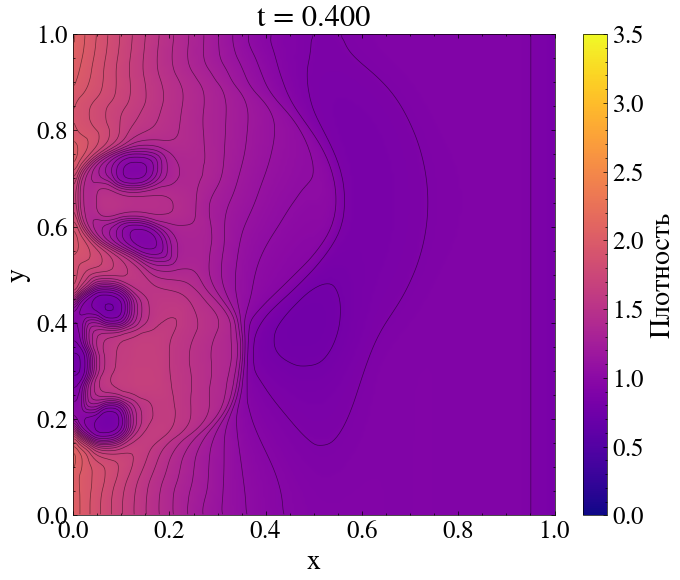
\includegraphics[width=\cellw]{rieman_modify_2d_final_jax_fd2.png} &
%					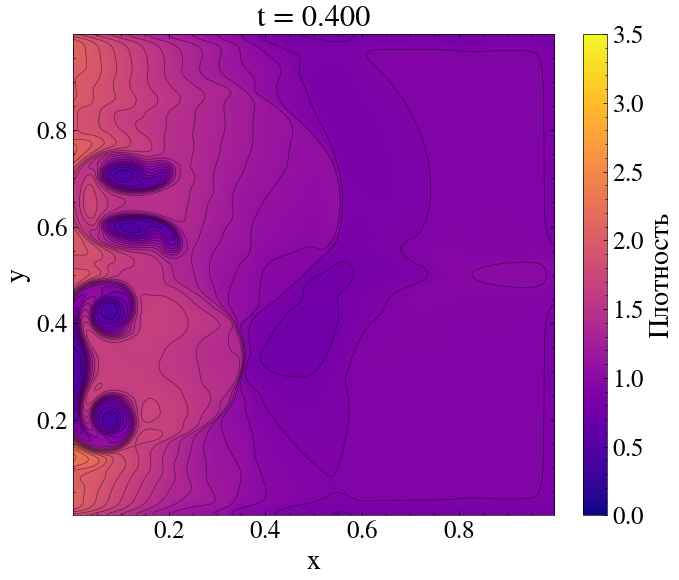
\includegraphics[width=\cellw]{rieman_modify_2d_final_jax-fluids.png} \\
%				\end{tabular}
%			\end{column}
%		\end{columns}
%		
%	\end{frame}

	\begin{frame}{Анализ сходимости в двумерной постановке}
	
	%--- ВЕРХ: два горизонтальных графика на всю ширину ---
	\vspace{-0.1cm}
	\begin{figure}[h]
		\centering
		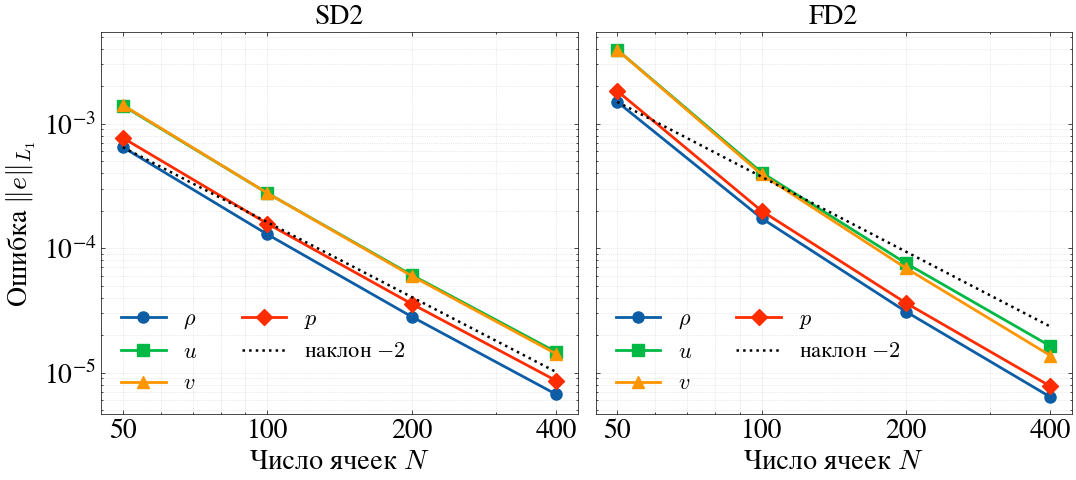
\includegraphics[width=0.65\textwidth]{convergence_2d_L1.png}
		\vspace*{-0.2cm}
		%
		\caption{\smaller{Ошибка по $\rho,p,u,v$ в норме $L_1$, 2D}}
	\end{figure}
	
	\vspace{-0.2cm}
	
	%--- НИЗ: слева Тест, справа Таблица порядков ---
	\begin{columns}[t]
		%--- ЛЕВО: описание теста ---
		\begin{column}{0.46\textwidth}
			\centering
			\footnotesize
			
			%				\vspace{0.5cm}
			\textbf{Тест:} перенос гладкого изоэнтропического вихря на области $[0,10]^2$ \\ с периодическими ГУ.
			%				\vspace{0.15cm}
			%				\begin{alertblock}{}
				%					\smaller \textbf{2-й порядок по всем переменным} и по обеим
				%					нормам. В отличие от 1D, $L_2$ \emph{не проседает} --- гладкий
				%					вихрь и неогранич. реконструкция.
				%				\end{alertblock}
		\end{column}
		
		%--- ПРАВО: таблица порядков ---
		\begin{column}{0.50\textwidth}
			\centering
			\vspace{-1cm}
			\begin{table}[h]
				\caption{\smaller{Эмпирический порядок сходимости $r$ ($N{:}\,200{\to}400$)}}
				\vspace{-0.3cm}
				\resizebox{0.6\textwidth}{!}{%
					\begin{tabular}{lcccc}
						\toprule
						\multirow{2}{*}{Перем.} & \multicolumn{2}{c}{SD2} & \multicolumn{2}{c}{FD2} \\
						\cmidrule(lr){2-3}\cmidrule(lr){4-5}
						& $r_{L_1}$ & $r_{L_2}$ & $r_{L_1}$ & $r_{L_2}$ \\
						\midrule
						$\rho$ & 2.07 & 2.06 & 2.28 & 2.29 \\
						$u$    & 2.06 & 2.08 & 2.21 & 2.26 \\
						$v$    & 2.08 & 2.09 & 2.33 & 2.38 \\
						$p$    & 2.05 & 2.07 & 2.22 & 2.30 \\
						\bottomrule
					\end{tabular}
				}
			\end{table}
		\end{column}
	\end{columns}
	
\end{frame}
	
	
	%==================================================================
	% Слайд: 2D плотность — начальное слева, сравнение методов справа
	\begin{frame}{Двумерная постановка: эволюция плотности}
		
		% Удобная длина для размера одной ячейки сетки справа
		\newlength{\cellw}\setlength{\cellw}{0.26\textwidth}
		
		\begin{columns}[c]
			%--- ЛЕВО: начальное условие (меньше) ---
			\begin{column}{0.22\textwidth}
				\centering
				\hspace*{-0.4cm}% <-- сдвиг графика влево
				\vspace{0.2cm}
%				\hspace*{-0.4cm}% <-- сдвиг графика влево
				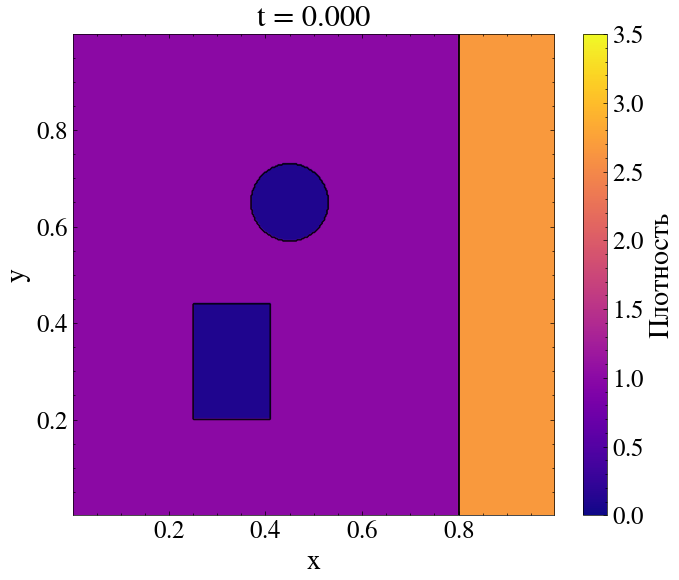
\includegraphics[width=1.2\textwidth]{rieman_modify_2d_init_jax-fluids.png}
				\hspace*{0.4cm}
				\text{\smaller{Начальное условие}}
			\end{column}
			
			%--- ПРАВО: сетка 2x3 (время x метод), крупнее ---
			\begin{column}{0.76\textwidth}
				\centering
				\setlength{\tabcolsep}{1pt}%
				\renewcommand{\arraystretch}{0.5}%
				\begin{tabular}{ccc}
					% --- строка 1: t = T/2 ---
					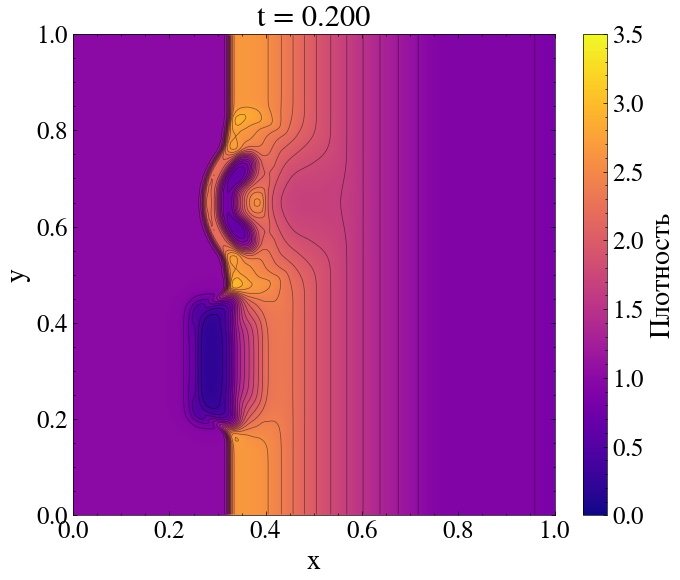
\includegraphics[width=\cellw]{rieman_modify_2d_half_jax_sd2.png} &
					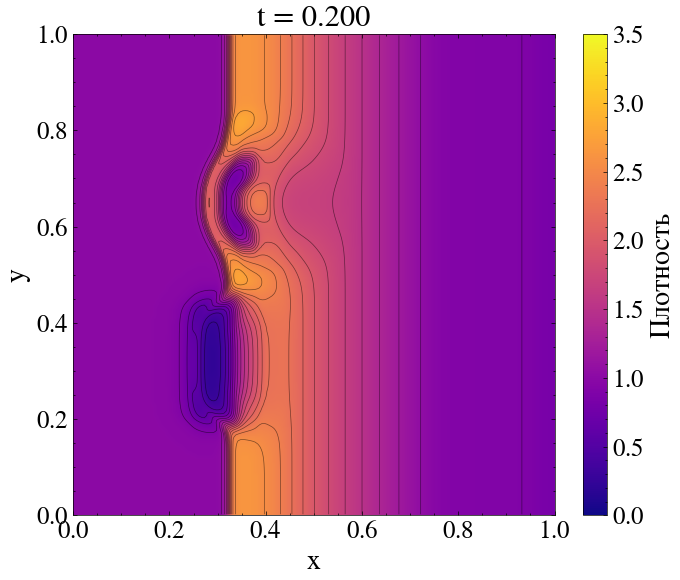
\includegraphics[width=\cellw]{rieman_modify_2d_half_jax_fd2.png} &
					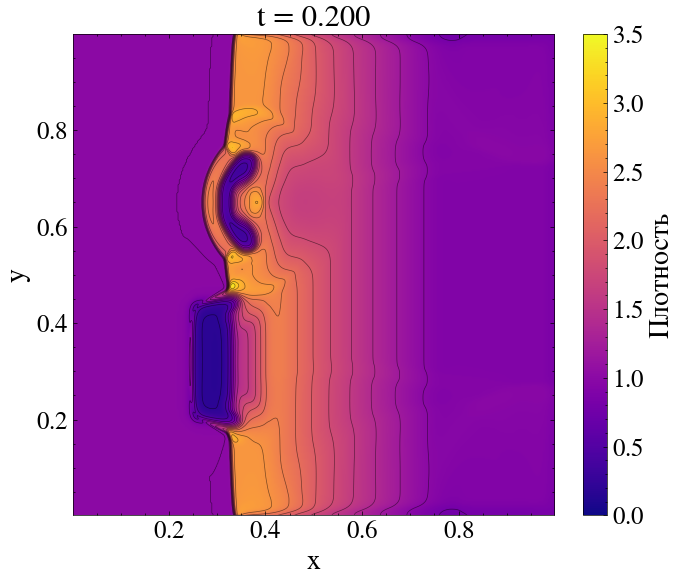
\includegraphics[width=\cellw]{rieman_modify_2d_half_jax-fluids.png} \\[2pt]
					% --- строка 2: t = T ---
					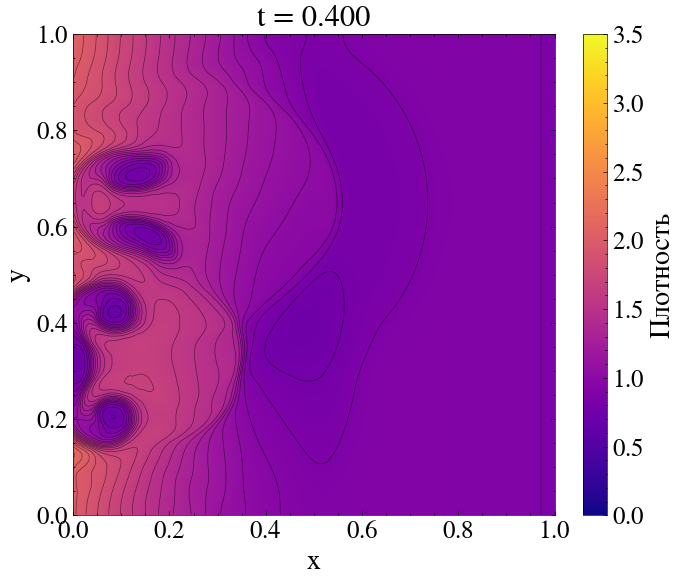
\includegraphics[width=\cellw]{rieman_modify_2d_final_jax_sd2.png} &
					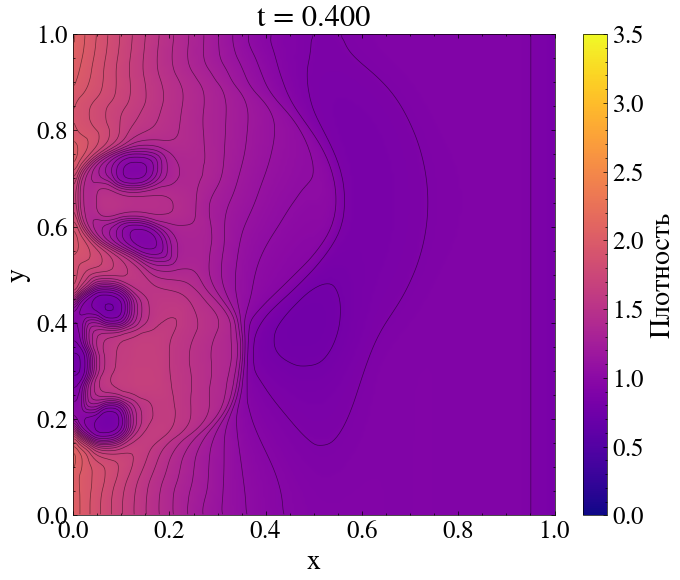
\includegraphics[width=\cellw]{rieman_modify_2d_final_jax_fd2.png} &
					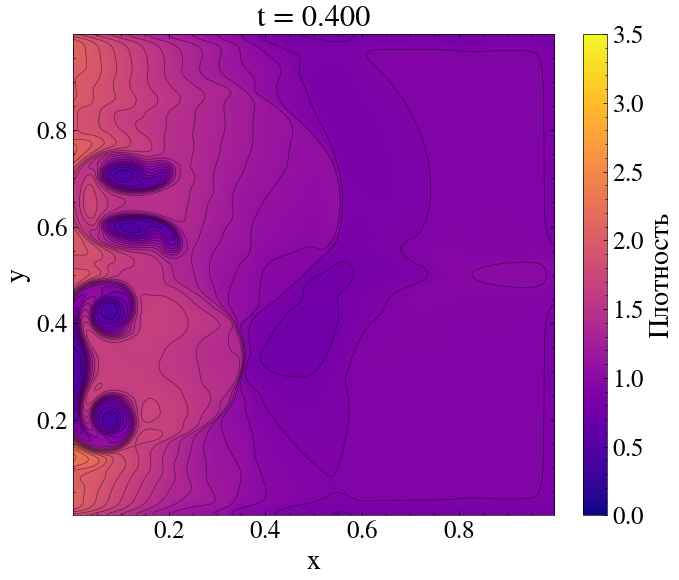
\includegraphics[width=\cellw]{rieman_modify_2d_final_jax-fluids.png} \\[2pt]
					% --- заголовки столбцов: методы ---
					SD2 & FD2 & JAX-FLUIDS \\
				\end{tabular}
			\end{column}
		\end{columns}
		
		\begin{center}
			{\smaller \textcolor{strucblue}{Рис.}~Эволюция плотности (эталон JAX-FLUIDS)}
		\end{center}
	
	\end{frame}
	
	
		%==================================================================

	%==================================================================
	% Слайд: Производительность (2D, схемы SD2 и FD2)
	\begin{frame}{Анализ аппаратного ускорения: двумерная постановка}
		
		\begin{columns}[c]
			\begin{column}{0.42\textwidth}
				\begin{figure}[h]
					\centering
					\vspace{-0.3 cm}
					\hspace*{-0.5cm}% <-- сдвиг графика влево
					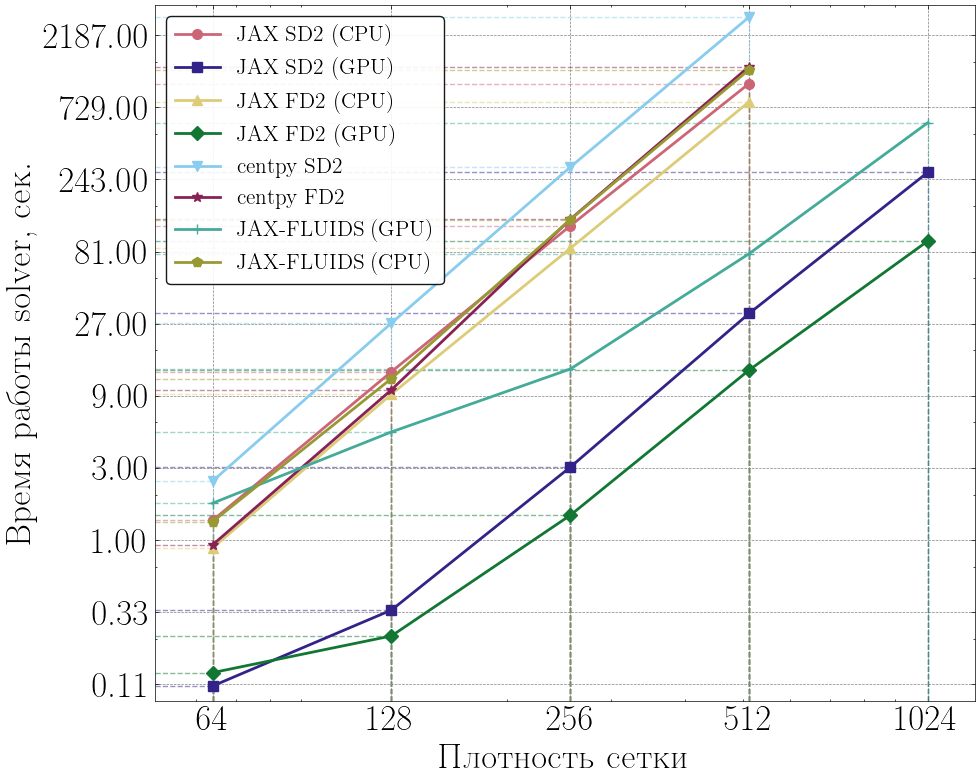
\includegraphics[width=1.12\textwidth]{compare_time_plot_2d.png}
					\caption{\smaller{Время счета (с), 2D}}
				\end{figure}
			\end{column}
			\begin{column}{0.58\textwidth}
				% ===== Основная таблица: SD2 + FD2 =====
				\begin{table}[h]
					\centering
					\caption{\smaller{Время счета (с), 2D, схемы SD2 и FD2}}
					\vspace{-0.2 cm}
					\resizebox{\textwidth}{!}{%
						\begin{tabular}{lcccccccc}
							\hline
							& \multicolumn{2}{c}{centpy}
							& \multicolumn{2}{c}{\tikzmark{tl2} \textbf{JAX CPU}}
							& \multicolumn{2}{c}{\textbf{JAX GPU}}
							& \multicolumn{2}{c}{JAX-FL.} \\
							$J\times J$ & SD2 & FD2 & \textbf{SD2} & \textbf{FD2} & \textbf{SD2} & \textbf{FD2} & CPU & GPU \\
							\hline
							$\mathbf{64}$   & 2.456    & 0.930    & \textbf{1.348}    & \textbf{0.885}   & \textbf{0.108}  & \textbf{0.133} & 1.322    & 1.753   \\
							$\mathbf{128}$  & 27.274   & 9.865    & \textbf{12.988}   & \textbf{9.233}   & \textbf{0.344}  & \textbf{0.232} & 11.709   & 5.191   \\
							$\mathbf{256}$  & 293.400  & 132.367  & \textbf{119.955}  & \textbf{85.072}  & \textbf{3.036}  & \textbf{1.458} & 131.803  & 13.530  \\
							$\mathbf{512}$ \tikzmark{br2} & 2888.498 & 1357.738 & \textbf{1047.884} & \textbf{793.620} & \textbf{31.572} & \textbf{13.316}& 1294.979 & 78.417  \\
							$\mathbf{1024}$ & ---      & ---      & ---      & ---     & \textbf{271.457}& \textbf{95.325}& ---      & 577.726 \\
							\hline
						\end{tabular}
					}
					\begin{tikzpicture}[remember picture, overlay]
						\draw[teal, very thick, rounded corners=2pt]
						([xshift=7pt, yshift=-14pt]pic cs:tl2) rectangle ([xshift=48pt, yshift=4pt]pic cs:br2);
					\end{tikzpicture}
				\end{table}
				
				\vspace{-0.2cm}
				% ===== Вторая таблица: ускорение Разраб. GPU =====
				\begin{table}[h]
					\centering
					\caption{\smaller{Ускорение JAX GPU (2D, $512\times512$)}}
					\vspace{-0.2 cm}
					\resizebox{0.85\textwidth}{!}{%
						\begin{tabular}{lcc}
							\hline
							Сравнение & SD2 & FD2 \\
							\hline
							JAX CPU        & 33.2$\times$          & 59.6$\times$  \\
							\tikzmark{tlc2} centpy  & \textbf{91.5$\times$ }         & \textbf{102.0$\times$} \tikzmark{brc2} \\
							JAX-FLUIDS GPU & 2.5$\times$           & 5.9$\times$            \\
							\hline
						\end{tabular}
					}
					\begin{tikzpicture}[remember picture, overlay]
						\draw[teal, very thick, rounded corners=2pt]
						([xshift=-7pt, yshift=10pt]pic cs:tlc2) rectangle ([xshift=8pt, yshift=-4pt]pic cs:brc2);
					\end{tikzpicture}
				\end{table}
			\end{column}
		\end{columns}
		
	\end{frame}
	
	
%		%==================================================================
%	% Слайд: Производительность (2D, схемы SD2 и FD2)
%	\begin{frame}{Сравнительный анализ аппаратного ускорения: двумерная постановка}
%		
%				\begin{columns}[c]
%			\begin{column}{0.36\textwidth}
%				\begin{figure}[h]
%					\centering
%					\vspace{-0.3 cm}
%					\hspace*{-0.8cm}% <-- сдвиг графика влево
%					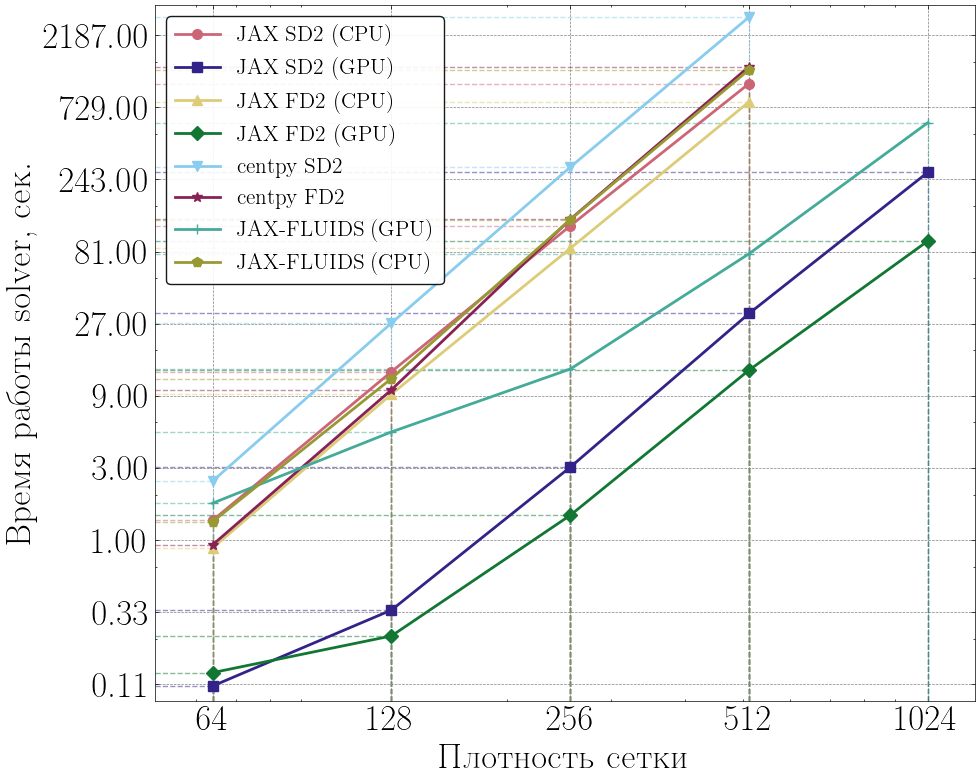
\includegraphics[width=1.22\textwidth]{compare_time_plot_2d.png}
%					\caption{\smaller{Время счёта (с) от размера сетки $J\times J$ (2D), лог-лог.}}
%				\end{figure}
%			\end{column}
%			\begin{column}{0.64\textwidth}
%				% ===== Основная таблица: SD2 + FD2 =====
%				\begin{table}[h]
%					\centering
%					\caption{\smaller{Время счёта (с), 2D, схемы SD2 и FD2}}
%					\vspace{-0.3 cm}
%					\setlength{\tabcolsep}{3pt}% <-- плотнее колонки => крупнее шрифт после resizebox
%					\resizebox{\textwidth}{!}{%
%						\begin{tabular}{lcccccccc}
%							\hline
%							& \multicolumn{2}{c}{\texttt{centpy}}
%							& \multicolumn{2}{c}{Разраб. CPU}
%							& \multicolumn{2}{c}{Разраб. GPU}
%							& \multicolumn{2}{c}{JAX-FL.} \\
%							$J\times J$ & SD2 & FD2 & SD2 & FD2 & SD2 & FD2 & CPU & GPU \\
%							\hline
%							$\mathbf{64}$   & 2.456    & 0.930    & 1.348    & 0.885   & \textbf{0.108}  & \textbf{0.133} & 1.322    & 1.753   \\
%							$\mathbf{128}$  & 27.274   & 9.865    & 12.988   & 9.233   & \textbf{0.344}  & \textbf{0.232} & 11.709   & 5.191   \\
%							$\mathbf{256}$  & 293.400  & 132.367  & 119.955  & 85.072  & \textbf{3.036}  & \textbf{1.458} & 131.803  & 13.530  \\
%							$\mathbf{512}$  & 2888.498 & 1357.738 & 1047.884 & 793.620 & \textbf{31.572} & \textbf{13.316}& 1294.979 & 78.417  \\
%							$\mathbf{1024}$ & ---      & ---      & ---      & ---     & \textbf{271.457}& \textbf{95.325}& ---      & 577.726 \\
%							\hline
%						\end{tabular}
%					}
%				\end{table}
%				
%				\vspace{-0.2cm}
%				% ===== Вторая таблица: ускорение Разраб. GPU =====
%				\begin{table}[h]
%					\centering
%					\caption{\smaller{Ускорение \texttt{JAX}. GPU (2D, $512\times512$)}}
%					\vspace{-0.3 cm}
%					\resizebox{0.85\textwidth}{!}{%
%						\begin{tabular}{lcc}
%							\hline
%							Сравнение & SD2 & FD2 \\
%							\hline
%							vs \texttt{JAX} CPU        & 33.2$\times$          & \textbf{59.6$\times$}  \\
%							vs \texttt{centpy}        & 91.5$\times$          & \textbf{102.0$\times$} \\
%							vs \texttt{JAX-FLUIDS} GPU & 2.5$\times$           & 5.9$\times$            \\
%							\hline
%						\end{tabular}
%					}
%				\end{table}
%			\end{column}
%		\end{columns}
%		
%	\end{frame}
	

	%==================================================================
	% Слайд: Заключение (синхронно с дипломом, верные числа, смягчено)
	\begin{frame}{Заключение и основные результаты}

		\begin{block}{Выводы}
			\begin{enumerate}
				\item Поставлена и решена модифицированная задача Римана о прохождении УВ через зону энерговложения для уравнений Эйлера (1D и 2D).
				\item Реализован высокопроизводительный комплекс на базе JAX (схемы SD2 и FD2): JIT-компиляция, векторизация, единый код для CPU и GPU без модификации.
				\item Подтвержден второй порядок точности на гладких решениях.
				\item Проведена верификация решения относительно открытой библиотеки JAX-FLUIDS: достигнуто хорошее согласие профилей.
				\item Относительно centpy разработанный комплекс на GPU быстрее до $47.9\times$ в одномерных задачах и в $90$–$100\times$ в двумерных; достигнута сетка $1024\times1024$.
			\end{enumerate}
		\end{block}

	\end{frame}

	%==================================================================
	% ВСПОМОГАТЕЛЬНЫЕ СЛАЙДЫ
	\appendix
	
	
	% TODO На слайде Как работае JAX можно добавить что такое JIT компиляция (в любой непонятной ситуации рассказывать про JIT компиляцию)
	
	% TODO Ренкино Гюгонио как получили числа для ударной волны
	
	% TODO Причесать нормы L1 и L2
	
	% TODO Расписать несколько лимитеров
	
	% TODO Расписать граничные условия и как они формулируются в коде
	
	% TODO Про шаг по времени и как он вычисляется в коде
	
	% TODO узнать про SSP2-RK2
	
	% TODO подробнее про шахматную сетку
	
%==================================================================
%==================================================================
% Appendix: нормы погрешности и порядок сходимости
	\begin{frame}{TVD-свойство}
	
	\begin{block}{TVD-свойство (Total Variation Diminishing)}
		Схема не порождает новые локальные экстремумы, если
		\vspace{-0.2 cm}
		\[
		TV(u^{n+1}) \leq TV(u^{n}),
		\]
		где общая вариация решения $TV(u) = \sum_{i = 1}^{N - 1} |u_{i + 1}(t) - u_i(t)|$
	\end{block}
	
	Для обеспечения TVD-свойства используются нелинейные ограничители наклонов (limiter):
	\vspace{-0.3 cm}
	\[
	\text{minmod}(a,b) = \frac{1}{2} \big( \operatorname{sgn}(a) + \operatorname{sgn}(b) \big) \cdot \min\big( |a|, |b| \big).
	\]
\end{frame}


\begin{frame}{Нормы погрешности $L_1$, $L_2$ и порядок сходимости}
	
	Для количественной оценки точности используются нормы $L_1$ и $L_2$.
	
	\vspace{0.2cm}
	\begin{columns}[t]
		\begin{column}{0.48\textwidth}
			\begin{block}{Норма $L_1$ --- интегральная погрешность}
				\[
				\|e\|_{L_1} = \frac{1}{N} \sum_{i=1}^{N}
				\left| u_i^h - u_i^{\mathrm{ref}} \right|
				\]
			\end{block}
		\end{column}
		\begin{column}{0.48\textwidth}
			\begin{block}{Норма $L_2$ --- среднеквадратическая}
				\[
				\|e\|_{L_2} = \sqrt{\frac{1}{N} \sum_{i=1}^{N}
					\left( u_i^h - u_i^{\mathrm{ref}} \right)^2}
				\]
			\end{block}
		\end{column}
	\end{columns}
	
	{\small где $u_i^h$ --- численное решение в центре $i$-й ячейки сетки
		из $N$ ячеек, $u_i^{\mathrm{ref}}$ --- точное аналитическое решение.}
	
	\vspace{0.2cm}
	\begin{block}{Эмпирический порядок сходимости (формула Ричардсона)}
		\[
		p = \log_2 \frac{\|e^{(N)}\|}{\|e^{(2N)}\|}
		\]
		\centering{\small при удвоении числа ячеек; теоретически для SD2 и FD2
			$p \approx 2$.}
	\end{block}
	
\end{frame}


\begin{frame}{Библиотека JAX}
	\begin{block}{Принцип работы JAX (конвейер JIT-компиляции)}
		\small
		\begin{enumerate}\itemsep2pt
			\item \textbf{Трассировка:} Python-функция выполняется с абстрактными (символьными) аргументами, в ходе чего фиксируется полная последовательность производимых операций.
			\item \textbf{Построение графа (\texttt{jaxpr}):} на основе трассировки формируется промежуточное представление программы --- граф вычислений.
			\item \textbf{Компиляция XLA:} граф вычислений компилируется средствами XLA в оптимизированный машинный код целевого устройства (CPU/GPU).
			\item \textbf{Исполнение и кэширование:} скомпилированное ядро исполняется на устройстве; результат компиляции сохраняется в кэше и повторно используется при последующих вызовах.
		\end{enumerate}
		%				\vspace{0.1cm}
		%				{\centering\footnotesize
			%					\texttt{f(x)} $\to$ трасса $\to$ \texttt{jaxpr} $\to$ XLA $\to$ ядро\par}
	\end{block}
\end{frame}

%	\begin{frame}{Аппаратное ускорение вычислений: фреймворк JAX}
%		Для преодоления вычислительных ограничений языка Python в качестве основы решателя выбран высокопроизводительный фреймворк JAX.
%
%		\vspace{0.3cm}
%		\textbf{Ключевые архитектурные преимущества:}
%		\begin{itemize}
%			\item \textbf{JIT-компиляция (Just-In-Time):} компилятор XLA (Accelerated Linear Algebra) транслирует высокоуровневый код Python в оптимизированные машинные инструкции.
%			\item \textbf{Глубокая векторизация:} отказ от явных циклов по пространственной сетке; массивы обрабатываются параллельно на уровне тензорных операций.
%			\item \textbf{Кроссплатформенность:} единый код (математическая логика решателя) нативно и без модификаций выполняется на многоядерных CPU и графических ускорителях (GPU/TPU).
%		\end{itemize}
%	\end{frame}

\begin{frame}{Программная реализация}
	\centering
	\vspace{0.3cm}
	
	Все алгоритмы реализованы в виде открытой библиотеки на Python\,/\,JAX.
	
	\vspace{0.25cm}
	Исходный код, примеры запуска и полное воспроизведение результатов
		работы доступны в GitHub-репозитории:
	
	\vspace{0.5cm}
%	\qrcode[height=3.2cm]{https://github.com/filkinc/diploma_centpy_parallelization_py}
	
	\vspace{0.5cm}
	{\large\url{https://github.com/filkinc/diploma_centpy_parallelization_py}}
\end{frame}


%	% Бэкап: 1D-производительность
%	\begin{frame}{Производительность: одномерная задача (бэкап)}
%		\begin{table}[h]
%			\centering
%			\footnotesize
%			\caption{\smaller{Время счета (с), 1D, схема SD2}}
%			\vspace{-0.2 cm}
%			\resizebox{\textwidth}{!}{%
%				\begin{tabular}{lccccc}
%					\hline
%					$J$ & \texttt{centpy} & Разраб. CPU & Разраб. GPU & JAX-FL. CPU & JAX-FL. GPU \\
%					\hline
%					$\mathbf{256}$   & 1.138   & 0.096   & \textbf{0.143}  & 0.954   & 3.894 \\
%					$\mathbf{512}$   & 4.244   & 0.394   & \textbf{0.179}  & 2.857   & 7.545 \\
%					$\mathbf{1024}$  & 5.577   & 2.499   & \textbf{0.370}  & 4.893   & 16.403 \\
%					$\mathbf{2048}$  & 16.175  & 7.255   & \textbf{0.720}  & 13.040  & 33.451 \\
%					$\mathbf{4096}$  & 41.613  & 29.928  & \textbf{1.500}  & 44.688  & 70.443 \\
%					$\mathbf{8192}$  & 152.440 & 86.862  & \textbf{3.931}  & 161.556 & 153.630 \\
%					$\mathbf{16384}$ & 612.826 & 349.892 & \textbf{12.805} & 633.204 & 404.548 \\
%					\hline
%				\end{tabular}
%			}
%		\end{table}
%		\centering\small
%		Ускорение GPU (1D, $J=16384$): $47.9\times$ относительно \texttt{centpy}, $27.3\times$ относительно собственной CPU-версии.
%		На малых 1D-сетках выигрыш GPU невелик из-за накладных расходов; преимущество раскрывается в 2D.
%	\end{frame}

\end{document}
